\documentclass[conference]{IEEEtran}
\IEEEoverridecommandlockouts

% Official unmodified IEEEtran packages
\usepackage{cite}
\usepackage{amsmath,amssymb,amsfonts,amsthm}
\usepackage{graphicx}
\usepackage{textcomp}
\usepackage{xcolor}
\usepackage{booktabs}
\usepackage{multirow}
\usepackage{array}
\usepackage{tabularx}
\usepackage{url}
\usepackage{balance}
\usepackage[hidelinks,bookmarks=false]{hyperref}

\newtheorem{proposition}{Proposition}

\def\BibTeX{{\rm B\kern-.05em{\sc i\kern-.025em b}\kern-.08em
    T\kern-.1667em\lower.7ex\hbox{E}\kern-.125emX}}

\begin{document}

\title{Crossing the Threshold: Mechanism and Ex-Ante Prediction of Local Explanation Instability in Credit Scoring}

\author{
\IEEEauthorblockN{Shahoud Shahid (23i-2515)}
\IEEEauthorblockA{\textit{School of Computing} \\
\textit{FAST--NUCES, Islamabad, Pakistan} \\
i232515@nu.edu.pk}
\and
\IEEEauthorblockN{Saif Shahzad (23i-2634)}
\IEEEauthorblockA{\textit{School of Computing} \\
\textit{FAST--NUCES, Islamabad, Pakistan} \\
i232634@nu.edu.pk}
}

\maketitle

\begin{abstract}
Local explainers such as SHAP and LIME underpin adverse-action reason codes in consumer credit scoring, yet minor input measurement noise can alter top-ranked attributions even when predicted default risk barely shifts. Extending the retraining benchmark of Ballegeer et al.\ (2025) across logistic regression, random forests, XGBoost, and instance-dependent cost-sensitive (\texttt{cslogit}, \texttt{csboost}) models on HMEQ, South German Credit (SGCS), and Taiwan Default, we unify across-refit replication with a fixed-model, prediction-preserving ($|\Delta p| \le 0.05$) mechanism and ex-ante fragility framework. Part~1 confirms monotonic instability rises as default prevalence drops ($30\%{\to}1\%$) in $38/40$ ($95.0\%$) cells and higher cost-sensitive instability in $64/80$ ($80.0\%$) comparisons, while variance decomposition proves $95.8\%$--$96.2\%$ of balanced-data LIME refit variance stems from explainer Monte Carlo noise rather than model retraining (vs.\ $4.1\%$--$34.3\%$ for PermutationSHAP). Under fixed models and $5\%$ input noise, exact TreeSHAP flips top-4 reasons in $23.5\%$--$92.3\%$ of prediction-preserving draws whereas LIME is masked beneath its unperturbed $95$th-percentile noise floor ($\bar{q}_{95} \in [0.358, 0.722]$) in $18/18$ cells. Joint regression across $48{,}547$ tree draws proves double dissociation: LIME flips track quantile-bin crossings ($\mathrm{OR}=1.361, p<10^{-8}$) rather than tree splits ($p=0.168$), while disabling discretisation cuts LIME instability by $83.4\%$ (HMEQ) and $82.1\%$ (SGCS). Finally, closed-form, perturbation-free fragility $F(x)$ beats tree-variance baselines on all datasets ($\Delta\mathrm{AUROC}=+0.112$ to $+0.184$) and flags HMEQ rejection \texttt{\#369} ($100\%$ flip rate).
\end{abstract}

\begin{IEEEkeywords}
Explainable artificial intelligence, credit scoring, SHAP, LIME, local explanation stability, threshold crossings, fragility prediction.
\end{IEEEkeywords}

% ==============================================================================
\section{Introduction}
\label{sec:intro}
% ==============================================================================
Financial institutions increasingly deploy tree ensembles alongside logistic regression to score consumer credit~\cite{ballegeer2025,baesens2016}. Under U.S.\ ECOA Regulation~B~\cite{regb_cfpb} and the EU AI Act~\cite{euaiact2024}, lenders issuing adverse credit decisions must furnish principal reason codes—typically top-$k$ features ($k=4$) ranked by SHAP~\cite{lundberg2017,lundberg2020} or LIME~\cite{ribeiro2016}. Yet credit bureau and borrower inputs carry minor measurement or rounding noise ($1$--$5\%$ spread) that can overturn reason codes even when a frozen model's predicted risk barely shifts ($|\Delta p| \le \tau$).

Building on Ballegeer et al.~\cite{ballegeer2025}, who benchmarked instance-dependent cost-sensitive (IDCS) credit models~\cite{bahnsen2014,vanderschueren2022b} across imbalance rates via LIME and permutation SHAP under bootstrap retraining, we move beyond across-refit turnover. Specifically, Ballegeer et al.\ evaluated retraining rather than fixed-model borrower perturbations, omitted exact TreeSHAP~\cite{lundberg2020}, and left inherent explainer sampling noise unseparated from genuine attribution shifts.

\textbf{Research Gap.} Despite recent XAI stability work~\cite{lin2025shap,bhuiyan2026,qi2026}, existing benchmarks neither isolate explainer Monte Carlo variance from prediction-preserving input instability under frozen credit models nor causally separate tree-split from discretisation-bin crossings, leaving lenders without a calibration-free ex-ante fragility score~\cite{hill2024,mikriukov2026}.

\textbf{Novelty.} Beyond retraining benchmarks~\cite{ballegeer2025}, we contribute: (i) an empirical noise-floor filter ($q_i$) paired with fixed-model, $\tau$-preserving ($0.05$) perturbations; (ii) a double-dissociation and discretisation-ablation test isolating threshold crossings ($C_{\mathrm{tree}}, C_{\mathrm{bin}}$) as the shared mechanism; and (iii) closed-form Gaussian fragility $F(x; s)$ requiring zero perturbations or hold-out calibration. Standard IDCS training~\cite{ballegeer2025,bahnsen2014} and credit datasets~\cite{baesens2016,sgcs2019,yeh2009} are adopted directly.

\textbf{Contributions.} This paper makes four contributions:
\begin{enumerate}
    \item \textit{Replicate and decompose retraining stability (H1a, H1b, E1):} Confirm monotonic instability increases as $\pi$ drops ($30\%{\to}1\%$) in $38/40$ ($95.0\%$) Holm-corrected cells and higher IDCS instability in $64/80$ ($80.0\%$) comparisons, while proving $95.8\%$--$96.2\%$ of balanced ($\pi{=}30\%$) LIME refit variance is explainer noise (vs.\ $4.1\%$--$34.3\%$ for PermSHAP).
    \item \textit{Separate sampling noise from structural shifts (H2--H3):} Show across 36 dataset--model--explainer--scale cells that exact TreeSHAP flips top-4 reasons in $23.5\%$--$92.3\%$ of $|\Delta p|\le 0.05$ draws, whereas LIME's high noise floor ($\bar{q}_{95}\in[0.358,0.722]$) masks input noise in $18/18$ cells ($p_{\mathrm{Holm}}{=}1.0$).
    \item \textit{Prove crossing double dissociation and causal mechanism (H4a--H4c):} Show across $48{,}547$ tree draws that LIME tracks bin crossings $C_{\mathrm{bin}}$ ($\mathrm{OR}{=}1.361, p_{\mathrm{Holm}}{=}2.0{\times}10^{-9}$, tree $p{=}0.168$) while TreeSHAP tracks $C_{\mathrm{tree}}$ ($\mathrm{OR}{=}1.091, p_{\mathrm{Holm}}{=}7.9{\times}10^{-21}$); disabling LIME discretisation cuts $\bar{U}_i$ by $83.4\%$ (HMEQ, $p{=}1.09{\times}10^{-13}$) and $82.1\%$ (SGCS, $p{=}2.62{\times}10^{-16}$).
    \item \textit{Derive and validate ex-ante fragility (H5--H6, R1--R9):} Validate closed-form $F(x)$, beating tree-variance baselines across all datasets ($\Delta\mathrm{AUROC}{=}{+}0.112$ to $+0.184$, $p{\le}5.9{\times}10^{-5}$; unweighted $F_{\mathrm{tree}}$ reaches $0.824$) and flagging HMEQ rejection \texttt{\#369} ($F_{\mathrm{tree}}{=}1.096$, $100\%$ TreeSHAP flips despite $p{=}0.9999$).
\end{enumerate}

Sections~II--IV review literature, theory, and research design; Sections~V--VI detail base--extended comparison and setup; Sections~VII--VIII report empirical and robustness results; Sections~IX--XI present the case study, limitations, and conclusions.

% ==============================================================================
\section{Literature Review and Hypotheses Development}
\label{sec:lit}
% ==============================================================================

\subsection{Retraining Instability and Cost-Sensitive Credit Scoring}
Post-hoc explainers such as LIME~\cite{ribeiro2016} and SHAP~\cite{lundberg2017,lundberg2020} translate credit-risk scores into adverse-action reason codes. While standard classifiers minimize symmetric cross-entropy, operational lending requires instance-dependent cost-sensitive (IDCS) losses reflecting exposure $A_i$, loss given default ($\mathrm{LGD}$), and foregone interest $r_i$~\cite{bahnsen2014,hoppner2022,vanderschueren2022b}. Benchmarking IDCS across resampled training folds, Ballegeer et al.~\cite{ballegeer2025} show via Coefficient of Variation ($\mathrm{CoV}$) and Sequential Rank Agreement ($\mathrm{SRA}$)~\cite{ekstrom2019} that severe class imbalance and cost-sensitive learning degrade attribution stability. Related credit and tabular studies corroborate retraining instability across imbalance rates~\cite{chen2024}, random seeds~\cite{lin2025shap,alkan2026}, and hyperparameter tuning~\cite{qi2026}, yet vary training data or seeds rather than perturbing inputs under a frozen model (motivating H1a--H1b).

\subsection{Explainer Stochasticity vs.\ Prediction-Preserving Perturbations}
Observed explanation turnover also confounds model sensitivity with explainer Monte Carlo variance. Sampling-based KernelSHAP~\cite{kelodjou2024} and tabular LIME~\cite{nnadi2026,zhou2021,visani2022,tzionis2026} produce different top-$k$ lists across repeated runs on the identical record. Notably, Ballegeer et al.~\cite{ballegeer2025} evaluate stochastic \texttt{PermutationExplainer}~\cite{strumbelj2014} and LIME without subtracting an empirical noise floor, conflating refit instability with sampling variance (motivating E1 and H2). Meanwhile, studies applying prediction-preserving input perturbations ($|\Delta p|\le\tau$) in software~\cite{hasnain2026}, fraud~\cite{bhuiyan2026}, and IoT~\cite{tolay2026} do not test noise-floor-controlled SHAP/LIME stability in credit scoring or assess whether $|\Delta p|$ reliably flags reason flips (motivating H3).

\subsection{Boundary Crossings and Ex-Ante Fragility Diagnostics}
Piecewise-constant geometry explains why minimal noise alters attributions: Pala and Garc\'{i}a-Cuesta~\cite{pala2024} prove RF-SHAP Lipschitz divergence at split crossings, Khan et al.~\cite{khan2024} link stability to probabilistic Lipschitzness and note discretised LIME violations, and Breeden~\cite{breeden2026} links boundary crossings to ``illusory explainability.'' However, no credit study tests split-threshold and bin-edge crossings as an instance-level mediator or establishes double dissociation between TreeSHAP and LIME (motivating H4a--H4c). Furthermore, existing instability gates require GP surrogates~\cite{hill2024}, ensemble variance~\cite{mikriukov2026}, or conformal calibration~\cite{breeden2026}, rather than a structure-only closed-form fragility score (motivating H5--H6).

\subsection{Gap-Based Literature Comparison and Research Gaps}
Table~\ref{tab:lit_gap} synthesizes 13 recent studies (2024--2026), including the base paper~\cite{ballegeer2025} and explicitly labeled preprints, alongside our proposed 2026 extension.

\begin{table*}[!t]
\centering
\caption{Gap-Based Literature Comparison Matrix (2024--2026)}
\label{tab:lit_gap}
\scriptsize
\renewcommand{\arraystretch}{0.82}
\setlength{\tabcolsep}{2.4pt}
\begin{tabular}{@{}p{1.9cm}cp{2.8cm}p{1.6cm}p{2.1cm}p{3.6cm}p{3.6cm}@{}}
\toprule
\textbf{Ref.} & \textbf{Year} & \textbf{Theory / Method} & \textbf{Context} & \textbf{Sample / Data} & \textbf{Key Findings} & \textbf{Limitations / Gap} \\
\midrule
Ballegeer et al.~\cite{ballegeer2025} (\textit{Base}) & 2025 & IDCS (\texttt{cslogit}, \texttt{csboost}) vs.\ CE; PermSHAP/LIME CoV/SRA & Credit scoring & 4 sets (HMEQ, SGCS, GMSC, VUB); $J{=}25$ & IDCS raises savings, cuts stability; worsens as $\pi{\le}5\%$ & Retraining only; no input noise, noise floor, or $F(x)$ (\textbf{G1--G4}) \\
Lin \& Wang~\cite{lin2025shap} & 2025 & 100-seed XGB retraining; Kendall's $W$ rank stability & Credit default & Taiwan ($30\text{k}{\times}23$) & Top-5 stable ($W{=}0.93$), mid-ranks volatile ($W{=}0.34$) & Seed refits on XGB only; no LIME/crossings (\textbf{G1, G3, G4}) \\
Bhuiyan et al.~\cite{bhuiyan2026} & 2026 & SHAP vs.\ PFI under dataset shift (LR, SVC, RF) & Fraud & BAF suite (6 variants) & SHAP ranks persist under shift while PFI drops & Dataset shift, not $\tau$-preserving input noise (\textbf{G1--G3}) \\
Qi et al.~\cite{qi2026} & 2026 & Multi-objective HPO for PR-AUC and SHAP CV stability & HR attrition & Tabular HR ensembles & Equal-accuracy models vary in SHAP stability & Training HPO; no fixed-model noise or $F(x)$ (\textbf{G1, G3, G4}) \\
Nnadi et al.~\cite{nnadi2026} & 2026 & Hierarchical H-LIME vs.\ LIME across repeated runs & Education & OULAD sparse logs & Standard LIME collapses ($\rho{\approx}0$) from run noise & No perturbation noise floor or bin mediation (\textbf{G1--G3}) \\
Tzionis et al.~\cite{tzionis2026} & 2026 & AKDE-LIME vs.\ LIME/TreeSHAP under 5--20\% noise & Energy & UCI Steel ($7$ feat.) & Adaptive KDE boosts LIME stability up to ${\sim}50{\times}$ & No $\tau$-filter, noise floor, or crossings (\textbf{G1--G4}) \\
Hasnain et al.~\cite{hasnain2026} & 2026 & Cross-method stability under $\tau$-preserving 1--5\% noise & Software & 5 AEEEM sets ($5{,}371$) & Preserving rate drops $89.2{\to}66.2\%$; Jaccard $0.78{\to}0.66$ & Software domain; no LIME floor removal or $F(x)$ (\textbf{G1--G4}) \\
Kelodjou et al.~\cite{kelodjou2024} & 2024 & Deterministic layer-wise neighbors (ST-SHAP) & Tabular XAI & HELOC, Boston, Bean & Eliminates KernelSHAP run variance ($\text{Jaccard}{=}1.0$) & Run noise only, not input noise or tree splits (\textbf{G1, G3, G4}) \\
Khan et al.~\cite{khan2024} & 2024 & Probabilistic Lipschitzness bounds on astuteness & Tabular/vision & Synthetic \& tabular & Proves bounds; discretised LIME lacks astuteness & Theoretical bounds; no credit crossing test (\textbf{G1, G3, G4}) \\
Mikriukov et al.~\cite{mikriukov2026} (\textit{Preprint}) & 2026 & Epistemic uncertainty gating for cost-aware XAI & Tabular/vision & Multi-domain benchmarks & Epistemic uncertainty negatively correlates with stability & Needs ensemble variance; no credit AUROC (\textbf{G1, G4}) \\
Tolay~\cite{tolay2026} (\textit{Preprint}) & 2026 & Prediction-preserving TreeSHAP stability and gating & IoT intrusion & CICIoT2023 ($39$ feat.) & XGB flips more than RF; gating saves 28--32\% & IoT; TreeSHAP only; no LIME, floor, or $F(x)$ (\textbf{G1--G4}) \\
Breeden~\cite{breeden2026} (\textit{Preprint}) & 2026 & Conformal uncertainty vs.\ boundary crossings & Credit \& risk & Conceptual benchmarks & Crossings create ``illusory explainability'' & Needs calibration set; no closed-form $F(x)$ (\textbf{G1, G3, G4}) \\
Pala \& Garc\'{i}a-Cuesta~\cite{pala2024} (\textit{Preprint}) & 2024 & Majority-tree SHAP averaging (AXOM) & Tabular XAI & Tabular RF benchmarks & Single split crossing causes Lipschitz divergence & RF+SHAP only; no XGB/LIME or mediation (\textbf{G1--G4}) \\
\midrule
\textbf{Proposed} & \textbf{2026} & \textbf{IDCS replication + noise-floor $\tau$-perturbations + crossing mediation + $F(x)$} & \textbf{Credit scoring} & \textbf{HMEQ, SGCS, Taiwan; LR, RF, XGB, IDCS} & \textbf{H1a 38/40, H1b 64/80; LIME 96\% noise; TreeSHAP 24--92\% flips; bin off $-82$--$83\%$; $F(x)$ $+\Delta$AUC 0.11--0.18} & \textbf{Gaps addressed: G1, G2, G3, G4} \\
\bottomrule
\end{tabular}
\end{table*}

Synthesizing Table~\ref{tab:lit_gap}, four gaps motivate our design: \textbf{G1} (lack of fixed-model, $\tau$-preserving credit perturbations across SHAP/LIME~\cite{ballegeer2025,lin2025shap}), \textbf{G2} (unseparated explainer sampling variance~\cite{ballegeer2025,nnadi2026}), \textbf{G3} (untested split- vs.\ bin-crossing mediation and double dissociation~\cite{pala2024,khan2024}), and \textbf{G4} (lack of a closed-form, calibration-free fragility score~\cite{mikriukov2026,breeden2026}).

% ==============================================================================
\section{Theoretical Background}
\label{sec:theory}
% ==============================================================================

\subsection{Classical Test Theory Lens on Explanation Reliability}
To ground empirical stability metrics in psychometric measurement theory, we model a local explainer applied to a frozen classifier $f$ as a measurement instrument evaluated under Classical Test Theory (CTT)~\cite{novick1966}. Under CTT, an observed attribution reading $\phi^{(k)}(x) = \phi_{\mathrm{true}}(x) + \varepsilon^{(k)}$ decomposes into a deterministic true attribution under the model's local functional behavior and a stochastic measurement error $\varepsilon^{(k)}$ induced by Monte Carlo coalition or neighborhood sampling~\cite{kelodjou2024,nnadi2026}. For deterministic exact explainers such as LinearSHAP and exact interventional TreeSHAP~\cite{lundberg2020}, $\mathrm{Var}(\varepsilon)=0$, yielding unit intraclass test--retest reliability $\mathrm{ICC}(1)=1.0$~\cite{shrout1979}. For stochastic explainers (\texttt{PermutationExplainer} and LIME), repeated draws on the unperturbed record $x$ quantify the empirical error distribution—the explainer's \textit{noise floor}. Because reliability bounds validity, any explanation change observed under a small input perturbation $x'$ signals genuine model-attribution instability only to the extent that it exceeds this noise floor.

\subsection{Piecewise-Constant Geometry and Boundary Crossings}
Whereas smooth linear scoring models exhibit continuous attribution sensitivity proportional to feature weights, tree ensembles (Random Forests~\cite{breiman2001} and XGBoost~\cite{chen2016}) and quantile-discretised tabular LIME~\cite{ribeiro2016} partition the feature space into hyper-rectangular regions bounded by axis-aligned split thresholds $\theta_n$ and discretiser cut-points $e \in E_j$. This geometry yields the sharp invariance property formalized in Proposition~\ref{prop:p1}:

\begin{proposition}[Piecewise Invariance Under Non-Crossing Perturbations]
\label{prop:p1}
Let $f$ be a trained tree ensemble with internal split thresholds $\{\theta_n\}$ and let $x, x' \in \mathbb{R}^D$ be two inputs.
\begin{enumerate}
    \item[(i)] For exact interventional TreeSHAP~\cite{lundberg2020} evaluated with a fixed background dataset, if $x_{j(n)}$ and $x'_{j(n)}$ lie on the same side of $\theta_n$ for every internal node $n$ in every tree $t$ (i.e., $C_{\mathrm{tree}}(x,x') = 0$), then every leaf routing across all coalitions is identical and $\phi^{\mathrm{TreeSHAP}}(x') = \phi^{\mathrm{TreeSHAP}}(x)$ exactly.
    \item[(ii)] For discretised tabular LIME~\cite{ribeiro2016} (verified in pinned \texttt{lime\_tabular} where \texttt{inverse[0]} holds $x$ and all perturbed neighbors are sampled conditional on discretised bin indices), if $x$ and $x'$ share identical bin indices across all features (i.e., $C_{\mathrm{bin}}(x,x') = 0$), the surrogate feature encoding is invariant except for the unperturbed reference row and Monte Carlo neighborhood noise, bounding expected attribution change at the explainer's noise floor.
\end{enumerate}
\end{proposition}

\noindent\textit{Proof sketch.} Interventional TreeSHAP evaluates each coalition $S$ by replacing missing coordinates with background draws while routing active features $j{\in}S$ via $\mathbb{I}[x_j \prec_n \theta_n]$. Under $C_{\mathrm{tree}}(x,x'){=}0$, $\mathbb{I}[x_{j(n)}{\prec_n}\theta_n]{=}\mathbb{I}[x'_{j(n)}{\prec_n}\theta_n]$ for all nodes, yielding identical coalition outputs and Shapley values. For discretised LIME, zero bin crossings preserve the binary indicator encoding around $x$, leaving only Monte Carlo sampling variance $\varepsilon$. $\square$

\subsection{Algorithmic Accountability in Consumer Credit}
Under U.S.\ ECOA Regulation~B~\cite{regb_cfpb} and the EU AI Act~\cite{euaiact2024}, adverse credit decisions require up to four accurate principal reasons and high-risk transparency oversight. When negligible noise flips top-4 reasons without altering risk scores, notices become arbitrary—motivating boundary-aware fragility gating. Table~\ref{tab:constructs} summarizes core constructs.

\begin{table}[!t]
\centering
\caption{Construct Definitions and Operational Sources}
\label{tab:constructs}
\scriptsize
\renewcommand{\arraystretch}{0.84}
\setlength{\tabcolsep}{2.4pt}
\begin{tabular}{@{}p{2.05cm}p{3.75cm}p{2.2cm}@{}}
\toprule
\textbf{Construct} & \textbf{Operational Definition} & \textbf{Source} \\
\midrule
Retraining instab. & Instance $\mathrm{CoV}$ and depth-$10$ $\mathrm{SRA}$ across $J$ refits & Ballegeer~\cite{ballegeer2025}; \cite{ekstrom2019} \\
Expl.\ change ($\Delta E$) & Top-4 Jaccard $D_k$ (primary); Spearman $D_\rho$; norm.\ $L_1$ ($D_1$) & Hasnain~\cite{hasnain2026}; \cite{lin2025shap} \\
Reason flip ($RC$) & Binary indicator $1[D_k(x,x') > q_i]$ above noise floor & Reg.\ B~\cite{regb_cfpb}; ours \\
Noise floor ($q_i$) & $95$th pct.\ of $D_k$ across $K{=}10$ seeds on unperturbed $x_i$ & CTT~\cite{novick1966}; \cite{kelodjou2024} \\
$\tau$-preserv.\ draw & Perturbed $x'$ with $\hat{y}(x')=\hat{y}(x)$ and $|p(x')-p(x)|\le\tau$ & Khan~\cite{khan2024}; \cite{tolay2026} \\
Perturb.\ scale ($s$) & Continuous-only noise $\delta_j \sim \mathcal{N}(0, (s\cdot\mathrm{SD}_j)^2)$ & Adapted from~\cite{tolay2026} \\
Crossings ($C_{\mathrm{tree}},C_{\mathrm{bin}}$) & Per-tree split or LIME bin-edge crossings ($x{\to}x'$) & \cite{pala2024,breeden2026} \\
Ex-ante $F(x)$ & Closed-form expected crossings under $\mathcal{N}(0,(s\cdot\mathrm{SD}_j)^2)$ & \textbf{Proposed (new)} \\
Cost-sensitivity & IDCS (\texttt{cslogit}, \texttt{csboost}) vs.\ CE (\texttt{logit}, \texttt{boost}) & Bahnsen~\cite{bahnsen2014}; \cite{hoppner2022} \\
Imbalance ($\pi$) & Training default rate $\pi \in \{1, 5, 10, 20, 30\}\%$ & Ballegeer~\cite{ballegeer2025} \\
\bottomrule
\end{tabular}
\end{table}

% ==============================================================================
\section{Conceptual Model and Research Design}
\label{sec:design}
% ==============================================================================

\subsection{Conceptual Framework and Methodology Pipeline}
Fig.~\ref{fig:conceptual_model} illustrates our integrated conceptual model linking the replicated base framework (left, blue) with the fixed-model, instance-level extension (right, green). In the base block, model class, cost-sensitivity (IDCS vs.\ standard cross-entropy), and training class imbalance ($\pi$) drive retraining instability ($\mathrm{CoV}$, $\mathrm{SRA}$). Estimation objective E1 bridges the two blocks by decomposing across-refit variance into genuine model variation versus explainer sampling noise. In the extension block, perturbation magnitude $s$ induces split-threshold ($C_{\mathrm{tree}}$) and bin-edge ($C_{\mathrm{bin}}$) crossings, which mediate local explanation change $\Delta E$ after controlling for the explainer noise floor $q_i$, moderated by explainer type and LIME discretisation. Prediction probability change $|\Delta p|$ acts only as a weak direct indicator of reason-code turnover (H3), whereas our structure-only fragility score $F(x)$ predicts unstable instances $Y_i$ ahead of any perturbation run (H5) and connects back to base-model factors (H6).

\begin{figure*}[!t]
\centering
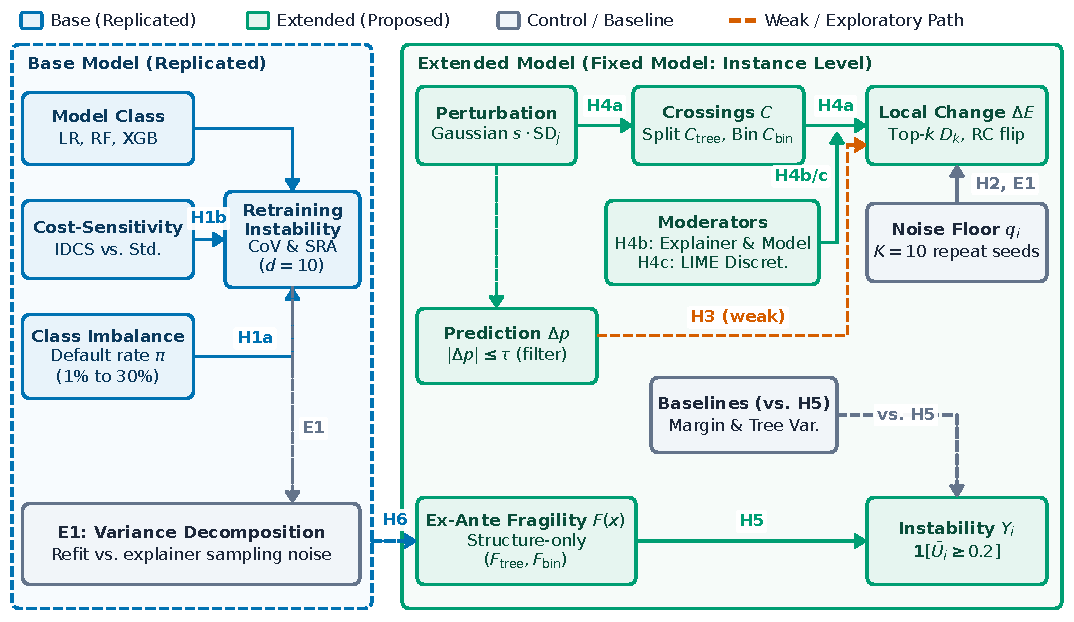
\includegraphics[width=0.46\textwidth]{figures/fig1_conceptual_model.pdf}
\caption{Integrated conceptual framework linking the replicated retraining-stability model of Ballegeer et al.~\cite{ballegeer2025} (left) with the proposed fixed-model crossing-mechanism and ex-ante fragility extension (right).}
\label{fig:conceptual_model}
\end{figure*}

Fig.~\ref{fig:methodology_flowchart} outlines the six-stage reproducible execution workflow: leak-free preparation (\texttt{01\_clean.py}), Part~1 replication and E1 decomposition (\texttt{02\_replicate.py}), fixed-model perturbation and fragility scoring (\texttt{03\_extend.py}), confirmatory and R1--R9 testing (\texttt{04\_robustness.py}), the HMEQ audit gate (\texttt{run\_demo.py}), and plotting (\texttt{05\_plots.py}).

\subsection{Pre-Registered Hypotheses}
Prior to executing main experimental runs, we locked the following directional hypotheses and estimation objective:
\begin{itemize}
    \item \textbf{H1a (Replication---Imbalance):} Across refits, instability ($\mathrm{CoV}$, $\mathrm{SRA}_{10}$) rises monotonically as default rate $\pi$ drops ($30\%{\to}1\%$).
    \item \textbf{H1b (Replication---IDCS):} Cost-sensitive models (\texttt{cslogit}, \texttt{csboost}) exhibit higher instability than standard baselines (\texttt{logit}, \texttt{boost}).
    \item \textbf{E1 (Variance Decomposition):} Quantify the share of across-refit variance caused by explainer noise vs.\ model retraining.
    \item \textbf{H2 (Noise-Floor Exceedance):} Under $|\Delta p|{\le}\tau$, $\Delta E$ exceeds $q_i$ for tree ensembles (TreeSHAP, LIME) and for LIME across models.
    \item \textbf{H3 (Weakness of $|\Delta p|$):} $|\Delta p|$ weakly discriminates $RC$ in trees (full-set AUROC upper CI $<0.70$~\cite{hosmer2013}), vs.\ stronger LR+LinearSHAP discrimination.
    \item \textbf{H4a (Crossing Mediation):} Crossing count $C$ ($C_{\mathrm{tree}}$ / $C_{\mathrm{bin}}$) mediates perturbation scale $s \to \Delta E$.
    \item \textbf{H4b (Double Dissociation):} TreeSHAP flips track $C_{\mathrm{tree}}$ ($\beta_{\mathrm{tree}}{>}0, \beta_{\mathrm{bin}}{\approx}0$); LIME flips track $C_{\mathrm{bin}}$ ($\beta_{\mathrm{bin}}{>}0, \beta_{\mathrm{tree}}{\approx}0$).
    \item \textbf{H4c (Discretisation Intervention):} Disabling LIME quantile discretisation reduces $\bar{U}_i$ among bin-crossing instances ($C_{\mathrm{bin}}{>}0$).
    \item \textbf{H5 (Ex-Ante Fragility):} $F(x)$ predicts unstable instances ($Y_i{=}1$) with higher AUROC than $B_{\mathrm{margin}}(x)$ and $B_{\mathrm{var}}(x)$.
    \item \textbf{H6 (Exploratory Bridge):} Crossings and $F(x)$ raise $R^2$ beyond base design factors, and IDCS yields higher mean $F(x)$.
\end{itemize}

\subsection{Mathematical Formulation and Notation}
Let $f: \mathbb{R}^D \to [0,1]$ denote a trained credit-default classifier outputting probability $p(x)$ and binary decision $\hat{y}(x) = \mathbb{I}[p(x) \ge t]$ at operating threshold $t$ (frozen to the training default prior $\hat{\pi}_1$). For an instance $x_i$ and perturbation scale $s$, we draw $R=25$ perturbations $x'_{ir} = \mathrm{clip}(x_i + \delta_{ir})$ where $\delta_{ir,j} \sim \mathcal{N}(0, (s\cdot\mathrm{SD}_j)^2)$ for continuous perturbable features ($\delta_{ir,j} = 0$ for categorical/discrete features), clipped to training $[0.5\text{th}, 99.5\text{th}]$ percentiles. A draw $x'_{ir}$ is retained as prediction-preserving ($r \in V_i$) iff it satisfies the tolerance rule in Eq.~\eqref{eq:filter}:
\begin{equation}
\label{eq:filter}
\hat{y}(x'_{ir}) = \hat{y}(x_i) \quad \text{and} \quad |p(x'_{ir}) - p(x_i)| \le \tau,
\end{equation}
with $\tau = 0.05$; non-preserving draws are preserved separately as the H3 contrast group to prevent range-restriction bias.

Let $\phi(x) \in \mathbb{R}^D$ denote the local attribution vector and $T_k(\phi(x))$ the top-$k$ feature indices ordered by $|\phi_j|$ ($k=4$~\cite{regb_cfpb}). Eqs.~\eqref{eq:dk}, \eqref{eq:dsec}, \eqref{eq:rc}, and \eqref{eq:instab} define primary explanation change $D_k$, secondary rank/magnitude distances ($D_\rho, D_1$), reason-code flip $RC_{ir}$, and instance instability label $Y_i$:
\begin{align}
D_k(x, x') &= 1 - \frac{|T_k(\phi(x)) \cap T_k(\phi(x'))|}{|T_k(\phi(x)) \cup T_k(\phi(x'))|}, \label{eq:dk} \\
D_\rho(x, x') &= 1 - \rho_S\big(\phi(x), \phi(x')\big), \nonumber \\
D_1(x, x') &= \frac{\|\phi(x') - \phi(x)\|_1}{\|\phi(x)\|_1 + \epsilon}, \label{eq:dsec} \\
RC_{ir} &= \mathbb{I}\big[D_k(x_i, x'_{ir}) > q_i\big], \label{eq:rc} \\
\bar{U}_i &= \frac{1}{|V_i|} \sum_{r \in V_i} RC_{ir}, \qquad
Y_i = \mathbb{I}\big[\bar{U}_i \ge 0.20\big], \label{eq:instab}
\end{align}
where $q_i$ is the $95$th percentile of $D_k$ across $\binom{K}{2}=45$ pairs from $K=10$ independent explainer seeds on unperturbed $x_i$ ($q_i=0$ for deterministic exact explainers).

For a tree ensemble with $T$ trees, internal nodes $N_t$, split features $j(n)$, thresholds $\theta_n$, and branching operator $\prec_n$ ($\le$ for \texttt{scikit-learn}, $<$ for \texttt{XGBoost}), and for LIME interior bin edges $E_j$, Eqs.~\eqref{eq:ctree}--\eqref{eq:cbin} define the empirical crossing counts:
\begin{align}
C_{\mathrm{tree}}(x, x') &= \frac{1}{T}\sum_{t=1}^T \sum_{n \in N_t} \mathbb{I}\big[\mathrm{side}_n(x_{j(n)}) \neq \mathrm{side}_n(x'_{j(n)})\big], \label{eq:ctree} \\
C_{\mathrm{bin}}(x, x') &= \sum_{j \in \mathcal{P}} \sum_{e \in E_j} \mathbb{I}\big[\mathbb{I}(x_j \le e) \neq \mathbb{I}(x'_j \le e)\big], \label{eq:cbin}
\end{align}
where $\mathrm{side}_n(z) = \mathbb{I}[z \prec_n \theta_n]$ and $\mathcal{P}$ denotes perturbable continuous features. Because $\delta_j \sim \mathcal{N}(0, \sigma_j^2)$ with $\sigma_j = s\cdot\mathrm{SD}_j$ is symmetric around zero, the marginal probability that $x_j + \delta_j$ crosses a threshold $\theta$ equals $\Phi(-|x_j - \theta|/\sigma_j)$, where $\Phi$ is the standard normal CDF. By linearity of expectation, without assuming feature or node independence, Eqs.~\eqref{eq:ftree}--\eqref{eq:fbin} yield the closed-form expected crossing counts:
\begin{align}
F_{\mathrm{tree}}^{\mathrm{unw}}(x; s) &= \frac{1}{T}\sum_{t=1}^T \sum_{n \in N_t,\, j(n)\in\mathcal{P}} \Phi\!\left(-\frac{|x_{j(n)} - \theta_n|}{s\cdot\mathrm{SD}_{j(n)}}\right), \label{eq:ftree} \\
F_{\mathrm{bin}}^{\mathrm{unw}}(x; s) &= \sum_{j \in \mathcal{P}} \sum_{e \in E_j} \Phi\!\left(-\frac{|x_j - e|}{s\cdot\mathrm{SD}_j}\right). \label{eq:fbin}
\end{align}
We also evaluate one pre-specified cover-weighted variant $F_{\mathrm{tree}}^{\mathrm{cov}}(x; s)$ multiplying each node $n$ by its training sample cover normalized by its tree's root cover, $w_n = \mathrm{cover}_n / \mathrm{cover}_{\mathrm{root}(t)}$, with no fitted weights. Against $F(x)$, we benchmark two perturbation-free baselines: decision margin $B_{\mathrm{margin}}(x) = -|p(x) - t|$ and RF epistemic prediction variance across trees $B_{\mathrm{var}}(x) = \mathrm{Var}_{t=1}^T(p_t(x))$~\cite{mikriukov2026}.

To test H4a, we estimate clustered linear mediation~\cite{preacher2008} separately per model--explainer pair via Eq.~\eqref{eq:med}:
\begin{equation}
\label{eq:med}
C_{ir} = a_0 + a\, s_r + u_i, \qquad \Delta E_{ir} = b_0 + c'\, s_r + b\, C_{ir} + v_i,
\end{equation}
computing $95\%$ confidence intervals for the indirect effect $a\cdot b$ via $5{,}000$ instance-clustered bootstrap resamples. For double dissociation (H4b), we fit the joint logistic regression in Eq.~\eqref{eq:dissoc} with instance-clustered sandwich standard errors:
\begin{equation}
\label{eq:dissoc}
\mathrm{logit}\,\mathbb{P}(RC_{ir} = 1) = \gamma_0 + \beta_{\mathrm{tree}}\, C_{\mathrm{tree},ir} + \beta_{\mathrm{bin}}\, C_{\mathrm{bin},ir}.
\end{equation}
Finally, for nested robustness and H6, we evaluate OLS regressions on instance instability $\bar{U}_i$ with HC3 standard errors as specified in Eq.~\eqref{eq:nested}:
\begin{equation}
\label{eq:nested}
\begin{aligned}
M_0 &: \text{design factors}, & M_1 &: M_0 + |\overline{\Delta p}|_i, \\
M_2 &: M_1 + \bar{C}_i, & M_3 &: M_2 + F_i.
\end{aligned}
\end{equation}
Table~\ref{tab:notation} consolidates all mathematical symbols used in Eqs.~\eqref{eq:filter}--\eqref{eq:nested} and Part~1 replication metrics.

\begin{table}[!t]
\centering
\caption{Summary of Mathematical Notation}
\label{tab:notation}
\scriptsize
\renewcommand{\arraystretch}{0.82}
\setlength{\tabcolsep}{3.0pt}
\begin{tabular}{@{}ll@{}}
\toprule
\textbf{Symbol} & \textbf{Definition} \\
\midrule
$x_i, x'_{ir}$ & Test instance $i$ and its $r$-th perturbed draw ($r=1\dots R$) \\
$p(x), \hat{y}(x), t$ & Predicted default probability, class decision, threshold ($\hat{\pi}_1$) \\
$\tau, s, \sigma_j$ & Probability shift tolerance ($0.05$), noise scale, $\sigma_j = s\cdot\mathrm{SD}_j$ \\
$\phi(x), T_k(\phi)$ & Local attribution vector and top-$k$ feature set ($k=4$) \\
$D_k, D_\rho, D_1$ & Top-$k$ Jaccard, Spearman, and normalized $L_1$ distances \\
$K, q_i$ & Noise-floor seed repeats ($10$) and $95$th percentile baseline \\
$RC_{ir}, \bar{U}_i, Y_i$ & Reason-code flip, instance flip rate, instability label ($\bar{U}_i \ge 0.20$) \\
$C_{\mathrm{tree}}, C_{\mathrm{bin}}$ & Empirical per-tree split and LIME bin-edge crossing counts \\
$F_{\mathrm{tree}}, F_{\mathrm{bin}}$ & Closed-form expected crossing counts (unweighted / cover) \\
$\Phi(\cdot), w_n$ & Standard normal CDF; normalized tree-node cover weight \\
$B_{\mathrm{margin}}, B_{\mathrm{var}}$ & Decision-margin and RF tree-variance baselines \\
$\pi, J, \mathrm{CoV}, \mathrm{SRA}$ & Training default rate, refits, CoV, and depth-10 SRA \\
$a\cdot b, \beta_{\mathrm{tree}}, \beta_{\mathrm{bin}}$ & Clustered indirect mediation effect and joint logistic slopes \\
\bottomrule
\end{tabular}
\end{table}

\subsection{Sampling, Statistical Power, and Data Collection Procedure}
Following Ballegeer et al.~\cite{ballegeer2025}, Part~1 reserves a fixed $N=300$ stratified test set per dataset and varies $\pi \in \{1, 5, 10, 20, 30\}\%$ at fixed pool size $\lfloor \#\text{defaults}_{\mathrm{train}}/0.30\rfloor$. Part~2 uses $70/30$ stratified splits (reusing the $300$-row SGCS test set) and draws $n=200$ test instances per dataset stratified $50/50$ by $\hat{y}(x)$, restoring population rates via inverse-probability weights. Exact a-priori power ($\rho=0.20, \alpha=0.05, 1-\beta=0.80$) requires $n_{\min}=193$ (achieved $0.8001$; Fisher-$z$ $n=194$), satisfied per dataset ($600$ pooled). All datasets~\cite{baesens2016,sgcs2019,yeh2009} use seed-locked pipelines with zero test leakage.

\begin{figure*}[!t]
\centering
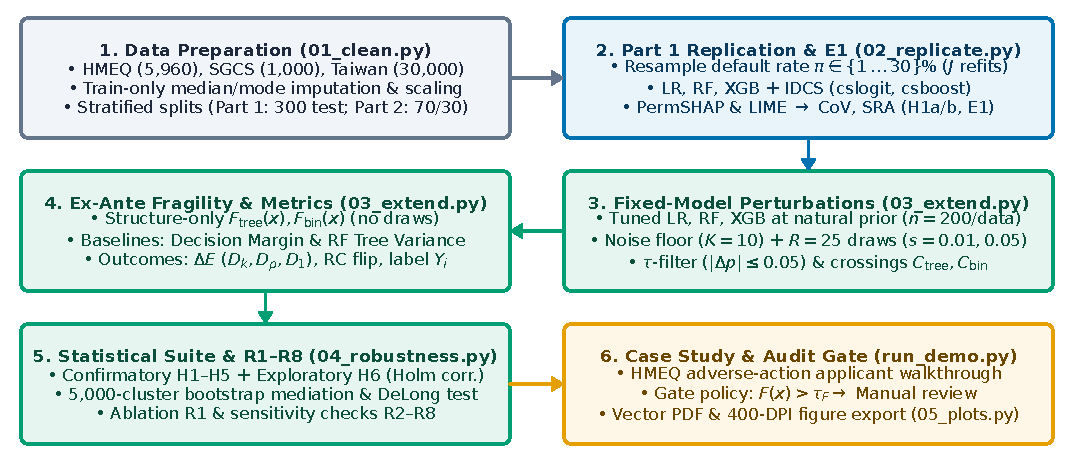
\includegraphics[width=0.46\textwidth]{figures/fig2_methodology_flowchart.pdf}
\caption{End-to-end six-stage research design and computational pipeline from raw credit data preprocessing to hypothesis testing, robustness ablation, and the adverse-action audit gate.}
\label{fig:methodology_flowchart}
\end{figure*}

% ==============================================================================
\section{Base vs. Extended Model Comparison}
\label{sec:comparison}
% ==============================================================================

Table~\ref{tab:base_vs_ext} contrasts the replicated base model of Ballegeer et al.~\cite{ballegeer2025} against our extended framework across theoretical constructs, perturbation mechanisms, and evaluation scope. Because several implementation details in~\cite{ballegeer2025} are unspecified in the published text, Appendix~\ref{app:tables} (Table~\ref{tab:deviations}) records all pre-registered alignment choices and justifiable scope deviations.

\begin{table*}[!t]
\centering
\caption{Side-by-Side Comparison of Base Model (Ballegeer et al., 2025) vs. Proposed Extended Model}
\label{tab:base_vs_ext}
\scriptsize
\renewcommand{\arraystretch}{0.82}
\setlength{\tabcolsep}{2.6pt}
\begin{tabular}{@{}p{2.3cm}p{6.5cm}p{7.6cm}@{}}
\toprule
\textbf{Dimension} & \textbf{Base Model (Ballegeer et al.~\cite{ballegeer2025})} & \textbf{Proposed Extended Model} \\
\midrule
Instability source & Model retraining across $J$ resampled pools & Fixed-model Gaussian noise ($\delta_j \sim \mathcal{N}(0,(s\cdot\mathrm{SD}_j)^2)$), $|\Delta p|\le\tau$ \\
Core predictors & Model class, IDCS vs.\ CE loss, default rate $\pi$ & Perturbation scale $s$, crossings ($C_{\mathrm{tree}}, C_{\mathrm{bin}}$), ex-ante $F(x)$, $|\Delta p|$ \\
Noise control & None (PermSHAP and LIME used unadjusted) & $K{=}10$ noise floor $q_i$ subtracted; E1 variance decomposition \\
Causal mechanism & None (descriptive CoV/SRA curves only) & Clustered mediation ($s{\to}C{\to}\Delta E$), double dissociation, LIME ablation \\
Ex-ante diagnostic & None & Closed-form $F_{\mathrm{tree}}(x)$ and $F_{\mathrm{bin}}(x)$ vs.\ margin/variance baselines \\
Outcome metrics & $\mathrm{CoV}$ and depth-$10$ $\mathrm{SRA}$ across refits & Noise-adjusted $D_k$ ($k{=}4$), $D_\rho$, $D_1$, flips $RC_{ir}$, label $Y_i$ \\
Datasets & GMSC, VUB (private), HMEQ, SGCS & HMEQ, SGCS (replicated) + Taiwan Default (independent main) \\
\bottomrule
\end{tabular}
\end{table*}

% ==============================================================================
\section{Data and Analysis Setup}
\label{sec:setup}
% ==============================================================================

\subsection{Datasets and Data Screening}
We evaluate three public credit-scoring datasets: two benchmarks replicated from Ballegeer et al.~\cite{ballegeer2025}---Home Equity (HMEQ)~\cite{baesens2016} and South German Credit (SGCS)~\cite{sgcs2019}---and an independent main sample, Taiwan Default of Credit Card Clients~\cite{yeh2009}. Table~\ref{tab:sample_profile} reports sample sizes, default prevalence, train/test partitions, and loan exposure columns ($A_i$). Because all data come from public archival credit records rather than surveys, the archival coverage rate is $100\%$.

\begin{table*}[!t]
\centering
\caption{Sample Profile and Partition Summary Across Credit Datasets}
\label{tab:sample_profile}
\scriptsize
\setlength{\tabcolsep}{3.5pt}
\begin{tabular}{@{}llrrrrrrrlr@{}}
\toprule
\textbf{Dataset} & \textbf{Role} & \textbf{Rows ($N$)} & \textbf{Feat.\ ($D$)} & \textbf{Perturb.} & \textbf{Defaults (\%)} & \textbf{Missing (\%)} & \textbf{Part~1 Split} & \textbf{Part~2 Split} & \textbf{Exposure ($A_i$)} & \textbf{Median (IQR)} \\
\midrule
HMEQ~\cite{baesens2016} & Base benchmark 1 & 5,960 & 12 & 6 & 1,189 (19.95) & 5,271 (7.37) & 5,660 / 300 & 4,172 / 1,788 & \texttt{LOAN} & 16,300 (12,200) \\
SGCS~\cite{sgcs2019} & Base benchmark 2 & 1,000 & 20 & 3 & 300 (30.00) & 0 (0.00) & 700 / 300 & 700 / 300 & \texttt{amount} & 2,320 (2,607) \\
Taiwan~\cite{yeh2009} & Independent main & 30,000 & 23 & 13 & 6,636 (22.12) & 0 (0.00) & 29,700 / 300 & 21,000 / 9,000 & \texttt{LIMIT\_BAL} & 140,000 (190,000) \\
\bottomrule
\end{tabular}
\end{table*}

Appendix~\ref{app:tables} (Table~\ref{tab:screening}) details feature screening: SGCS and Taiwan have zero missing values, whereas HMEQ has $5{,}271$ missing cells ($7.37\%$, led by \texttt{DEBTINC} $21.26\%$, \texttt{DEROG} $11.88\%$, \texttt{DELINQ} $9.73\%$). Continuous variables are strongly right-skewed (e.g., HMEQ \texttt{VALUE} skew $3.05$, SGCS \texttt{amount} $1.95$, Taiwan \texttt{PAY\_AMT2} $30.45$); outliers are retained for credit realism, motivating non-parametric rank tests and cluster bootstraps. Only continuous features are perturbed, while categorical/count variables stay fixed.

\subsection{Tool Justification, Configuration, and Evaluation Criteria}
We use script-based Python~3.11.4 (Table~\ref{tab:config}, Appendix~\ref{app:tables}) to access model tree splits, custom IDCS optimization, and seed-locked unit tests unavailable in menu-driven tools. Preprocessing is fitted strictly on training folds. Predictive quality uses ROC-AUC, AP, Brier score, and Savings/relAEC~\cite{ballegeer2025}; Part~1 stability uses $\mathrm{CoV}$ and $\mathrm{SRA}(10)$~\cite{ekstrom2019}; Part~2 uses noise-adjusted $D_k$ (Eq.~\eqref{eq:dk}), $RC_{ir}$ (Eq.~\eqref{eq:rc}), $Y_i$ (Eq.~\eqref{eq:instab}), the $\mathrm{AUROC}<0.70$ criterion for H3~\cite{hosmer2013}, and DeLong's test~\cite{delong1988} for H5.

% ==============================================================================
\section{Results and Discussion}
\label{sec:results}
% ==============================================================================

\subsection{Part~1 Replication: Imbalance, IDCS, and Variance Decomposition}
\label{sec:res_part1}
Replicating Ballegeer et al.~\cite{ballegeer2025} across five imbalance rates ($\pi \in \{1, 5, 10, 20, 30\}\%$, $J{=}10$ refits) supports H1a in $38/40$ ($95.0\%$) Holm-corrected cells ($19/20$ $\mathrm{CoV}$, $19/20$ $\mathrm{SRA}$; Fig.~\ref{fig:replication_curves}, Table~\ref{tab:replication_summary}). On HMEQ ($20/20$), lowering $\pi$ from $30\%$ to $1\%$ elevates $\mathrm{CoV}$ by $1.24\times$--$2.53\times$ and $\mathrm{SRA}(10)$ by $1.48\times$--$3.21\times$ ($\tau \in [-0.886, -0.594]$, $p_{\mathrm{Holm}} \le 3.05\times 10^{-174}$). On SGCS ($18/20$), $\mathrm{SRA}$ climbs $9.17\times$ for \texttt{boost}+LIME ($16.30{\to}149.50$) and $14.79\times$ for \texttt{csboost}+PermSHAP ($7.38{\to}109.06$); only \texttt{sgcs} \texttt{cslogit}+PermSHAP is non-significant ($\tau{=}{+}0.105, p_{\mathrm{Holm}}{=}1.0$; $\tau{=}{-}0.032, p_{\mathrm{Holm}}{=}0.065$) due to \texttt{cslogit} collapse ($\mathrm{AUC}{=}0.486$, $\mathrm{CoV}{=}0.000$) at $\pi{=}1\%$.

H1b holds in $64/80$ ($80.0\%$) Wilcoxon tests ($33/40$ $\mathrm{CoV}$, $31/40$ $\mathrm{SRA}$): \texttt{cslogit} exceeds \texttt{logit} instability in $38/40$ ($95.0\%$) cells ($r \in [0.608, 1.000]$), while \texttt{csboost} exceeds \texttt{boost} in $26/40$ ($65.0\%$, led by SGCS $16/20$ and HMEQ PermSHAP $8/10$). Crucially, E1 decomposition ($K{=}5$, $5{,}000$ bootstraps on SGCS; Table~\ref{tab:replication_summary}) shows PermSHAP variance is refit-driven ($\mathrm{ICC}{=}0.657$--$0.959$; explainer share $4.1\%$--$34.3\%$), whereas at $\pi{=}30\%$, \textbf{explainer noise accounts for $95.8\%$ (\texttt{logit}) and $96.2\%$ (\texttt{boost}) of LIME refit variance} ($\mathrm{ICC}\le 0.042$). At $\pi{=}1\%$, refit variance surges $49\times$ (\texttt{logit}: $0.34{\to}16.56$) and $14\times$ (\texttt{boost}: $0.12{\to}1.73$), reducing LIME's explainer share to $41.4\%$ and $36.0\%$.

\begin{figure*}[!t]
\centering
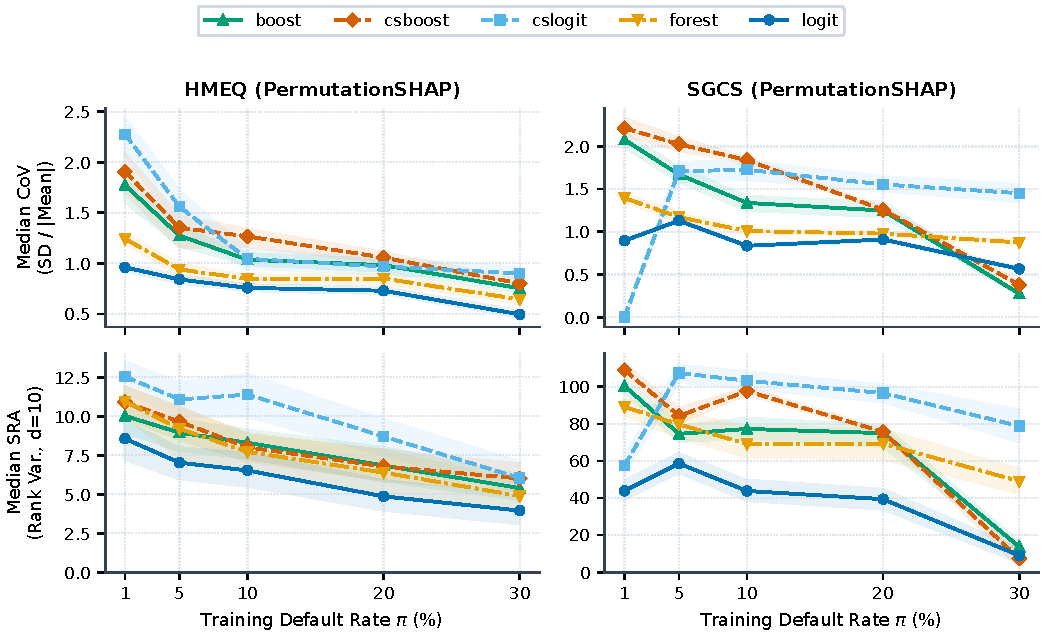
\includegraphics[width=0.47\textwidth]{figures/fig3_replication_curves.pdf}
\caption{Part~1 retraining stability replication across training default rates $\pi \in \{1, 5, 10, 20, 30\}\%$ ($J{=}10$ refits, PermutationSHAP median $\pm$ IQR): lower prevalence and IDCS (\texttt{cslogit}, \texttt{csboost}) monotonically increase $\mathrm{CoV}$ and $\mathrm{SRA}(10)$, save for \texttt{cslogit} collapse at SGCS $\pi{=}1\%$.}
\label{fig:replication_curves}
\end{figure*}

\begin{table}[!t]
\centering
\caption{Part~1 Replication Summary (H1a, H1b) and E1 Variance Decomposition (SGCS)}
\label{tab:replication_summary}
\scriptsize
\renewcommand{\arraystretch}{0.84}
\setlength{\tabcolsep}{2.6pt}
\resizebox{\columnwidth}{!}{%
\begin{tabular}{@{}llrrrr@{}}
\toprule
\multicolumn{6}{l}{\textbf{Panel A: Confirmatory Part~1 Counts (Holm--Bonferroni $\alpha=0.05$)}} \\
\textbf{Test} & \textbf{Scope} & \textbf{CoV} & \textbf{SRA} & \textbf{Total} & \textbf{Min--Max Effect} \\
\midrule
H1a Trend & HMEQ / SGCS & 19/20 & 19/20 & 38/40 & $\tau \in [-0.989, +0.105]$ \\
H1b \texttt{cslogit} & vs.\ \texttt{logit} & 18/20 & 20/20 & 38/40 & $r \in [-1.000, +1.000]$ \\
H1b \texttt{csboost} & vs.\ \texttt{boost} & 15/20 & 11/20 & 26/40 & $r \in [-0.969, +1.000]$ \\
\midrule
\multicolumn{6}{l}{\textbf{Panel B: E1 Nested Variance Decomposition (SGCS, $J{=}10, K{=}5$)}} \\
\textbf{Model--Expl.} & \textbf{$\pi$} & \textbf{Exp.\ Share} & \textbf{Refit ICC} & $\sigma^2_{\mathrm{exp}}$ & $\sigma^2_{\mathrm{refit}}$ \\
\midrule
\texttt{logit}--PermSHAP & 1\% / 30\% & 0.343 / 0.264 & 0.657 / 0.736 & 3.28 / 0.48 & 6.27 / 1.34 \\
\texttt{boost}--PermSHAP & 1\% / 30\% & \textbf{0.067} / \textbf{0.041} & 0.933 / 0.959 & 0.03 / 0.02 & 0.43 / 0.45 \\
\texttt{logit}--LIME & 1\% / 30\% & 0.414 / \textbf{0.958} & 0.586 / 0.042 & 11.69 / 7.59 & 16.56 / 0.34 \\
\texttt{boost}--LIME & 1\% / 30\% & 0.360 / \textbf{0.962} & 0.640 / 0.038 & 0.97 / 3.04 & 1.73 / 0.12 \\
\bottomrule
\end{tabular}}
\end{table}

\subsection{Predictive Baselines and Measurement Quality}
\label{sec:res_mq}
Part~2 predictive and economic baselines (detailed alongside Ballegeer et al.~\cite{ballegeer2025} averages in Appendix~\ref{app:tables}, Table~\ref{tab:model_perf}) confirm expected model ordering: \texttt{xgb} and \texttt{rf} outperform \texttt{lr} on discrimination (HMEQ AUC $0.964/0.960$ vs.\ $0.782$; Taiwan $0.777/0.775$ vs.\ $0.716$; SGCS $0.770/0.766$ vs.\ $0.743$), while IDCS variants (\texttt{cslogit}, \texttt{csboost}) trade AUC and Brier calibration for higher economic savings at the prior threshold (e.g., Taiwan \texttt{csboost} savings $0.411$ vs.\ \texttt{xgb} $0.331$; \texttt{cslogit} $0.323$ vs.\ \texttt{lr} $0.184$; SGCS \texttt{csboost} $0.350$ vs.\ \texttt{xgb} $0.294$).

Because survey SEM metrics (Cronbach's $\alpha$, CR, AVE) do not apply to computational explainers, Table~\ref{tab:measurement_quality} reports the pre-registered psychometric measurement analogues across all 18 dataset--model--explainer cells. Exact LinearSHAP and TreeSHAP achieve perfect test--retest reliability ($\mathrm{ICC}(1)=1.000$, noise floor $q_{95}=0.000$). By contrast, LIME exhibits substantial run-to-run sampling noise even on unperturbed records ($\bar{q}_{95} \in [0.358, 0.722]$, $\mathrm{ICC}(1) \in [0.489, 0.828]$), meaning repeated LIME runs already disagree on roughly half of the top-4 features without any input perturbation. Convergent validity between $D_\rho$ and $D_1$ is moderate to strong ($\rho \in [0.467, 0.927]$), and discriminant validity ($\mathrm{HTMT} < 0.85$) passes in $17/18$ cells (failing only on SGCS \texttt{xgb}+TreeSHAP at $\mathrm{HTMT}=0.969$, where probability steps track leaf attribution shifts). Independent seeds eliminate common-method seed artifacts.

\begin{table}[!t]
\centering
\caption{Measurement Quality Analogues Across Model--Explainer Cells}
\label{tab:measurement_quality}
\scriptsize
\renewcommand{\arraystretch}{0.88}
\setlength{\tabcolsep}{2.2pt}
\resizebox{\columnwidth}{!}{%
\begin{tabular}{@{}llrrrrr@{}}
\toprule
\textbf{Data} & \textbf{Model--Expl.} & $\bar{q}_{95}$ & $\mathrm{ICC}(1)$ & $\rho(D_\rho,D_1)$ & $\mathrm{HTMT}$ & \textbf{Pass} \\
\midrule
HMEQ & \texttt{lr}--LIME / LinSHAP & 0.383 / \textbf{0.000} & 0.820 / \textbf{1.000} & 0.574 / 0.498 & 0.145 / 0.640 & Yes / Yes \\
HMEQ & \texttt{rf}--LIME / TreeSHAP & 0.423 / \textbf{0.000} & 0.765 / \textbf{1.000} & 0.650 / 0.721 & 0.060 / 0.670 & Yes / Yes \\
HMEQ & \texttt{xgb}--LIME / TreeSHAP & 0.470 / \textbf{0.000} & 0.706 / \textbf{1.000} & 0.586 / 0.836 & 0.112 / 0.659 & Yes / Yes \\
\midrule
SGCS & \texttt{lr}--LIME / LinSHAP & 0.661 / \textbf{0.000} & 0.593 / \textbf{1.000} & 0.686 / 0.467 & 0.022 / 0.748 & Yes / Yes \\
SGCS & \texttt{rf}--LIME / TreeSHAP & 0.506 / \textbf{0.000} & 0.742 / \textbf{1.000} & 0.743 / 0.847 & 0.083 / 0.802 & Yes / Yes \\
SGCS & \texttt{xgb}--LIME / TreeSHAP & 0.358 / \textbf{0.000} & 0.828 / \textbf{1.000} & 0.708 / 0.927 & 0.090 / 0.969 & Yes / No \\
\midrule
Taiwan & \texttt{lr}--LIME / LinSHAP & 0.425 / \textbf{0.000} & 0.786 / \textbf{1.000} & 0.679 / 0.636 & 0.022 / 0.718 & Yes / Yes \\
Taiwan & \texttt{rf}--LIME / TreeSHAP & 0.676 / \textbf{0.000} & 0.547 / \textbf{1.000} & 0.735 / 0.792 & 0.144 / 0.533 & Yes / Yes \\
Taiwan & \texttt{xgb}--LIME / TreeSHAP & 0.722 / \textbf{0.000} & 0.489 / \textbf{1.000} & 0.728 / 0.850 & 0.043 / 0.763 & Yes / Yes \\
\bottomrule
\end{tabular}}
\end{table}

\subsection{Noise-Floor Exceedance (H2) and Probability-Shift Signals (H3)}
\label{sec:res_h2h3}
Evaluating H2 across 36 dataset--model--explainer--scale cells reveals a sharp dichotomy between exact and stochastic explainers (supported in $18/36$ cells overall, $12/12$ tree+TreeSHAP cells; Fig.~\ref{fig:perturbation_vs_floor}). For exact TreeSHAP ($q_i=0$), prediction-preserving perturbations ($s=0.05$) flip top-4 reason codes in a large majority of instances: $92.3\%$ ($95\%$ Clopper--Pearson CI $[87.7, 95.7]\%$, mean $\bar{U}_i=0.632$) on Taiwan \texttt{rf}, $82.7\%$ ($[76.6, 87.7]\%$, mean $0.489$) on Taiwan \texttt{xgb}, $72.9\%$ ($[65.5, 79.5]\%$, mean $0.304$) on HMEQ \texttt{rf}, $84.6\%$ ($[78.4, 89.6]\%$, mean $0.521$) on HMEQ \texttt{xgb}, $61.0\%$ ($[53.9, 67.8]\%$, mean $0.197$) on SGCS \texttt{rf}, and $23.5\%$ ($[17.8, 30.0]\%$, mean $0.076$) on SGCS \texttt{xgb}. Even LinearSHAP exhibits nonzero flip proportions ($2.0\%$--$31.0\%$ at $s=0.05$), though mean $\bar{U}_i$ remains low ($0.005$--$0.080$). Conversely, LIME fails the one-sided Wilcoxon exceedance test in $18/18$ cells ($p_{\mathrm{Holm}}=1.0$, rank-biserial $r \in [-0.985, -0.619]$): because LIME's unperturbed $95$th-percentile noise floor ($q_{95} \in [0.400, 0.667]$) exceeds typical perturbation distances (median $D_k \in [0.144, 0.520]$), small input noise is largely submerged beneath LIME's own Monte Carlo variance.

\begin{figure*}[!t]
\centering
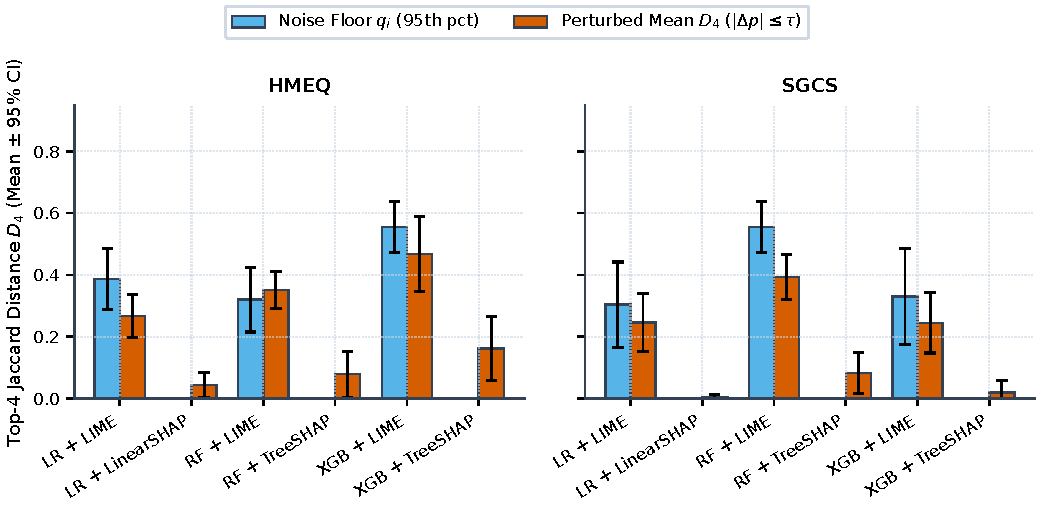
\includegraphics[width=0.49\textwidth]{figures/fig4_perturbation_vs_floor.pdf}
\caption{Unperturbed $95$th-percentile explainer noise floor $q_i$ vs.\ perturbed top-4 Jaccard distance $D_4$ ($|\Delta p| \le \tau$, $s{=}0.05$, mean $\pm 95\%$ CI). Exact SHAP baselines have zero noise floor and clear perturbation shifts, whereas LIME's sampling floor dominates perturbation-induced changes.}
\label{fig:perturbation_vs_floor}
\end{figure*}

For H3, we test $|\Delta p|$ discrimination of $RC_{ir}$ ($5{,}000$ cluster bootstraps) on full (primary) and $\tau$-filtered draws. \textbf{LIME} yields full-set AUROC upper CI $<0.70$ in $5/6$ tree cells ($0.473$--$0.572$; HMEQ \texttt{rf} $0.679$ $[0.610,0.746]$), whereas \textbf{TreeSHAP fails H3} ($0/6$ cells $<0.70$): full-set AUROCs reach $0.801$ $[0.769,0.832]$ (HMEQ \texttt{rf}), $0.740$ $[0.707,0.773]$ (HMEQ \texttt{xgb}), $0.777$ $[0.736,0.817]$ (SGCS \texttt{rf}), $0.959$ $[0.942,0.973]$ (SGCS \texttt{xgb}), $0.677$ $[0.643,0.709]$ (Taiwan \texttt{rf}), and $0.747$ $[0.715,0.777]$ (Taiwan \texttt{xgb}). Filtering attenuates $|\Delta p|$ AUROC (HMEQ \texttt{rf} $0.801{\to}0.681$; Taiwan \texttt{rf} $0.677{\to}0.629$), confirming range restriction while showing multi-split crossings shift $p(x)$. Fig.~\ref{fig:roc_comparison} contrasts this post-hoc $|\Delta p|$ baseline against ex-ante $F(x)$ in Section~\ref{sec:res_h5h6}.

\begin{figure*}[!t]
\centering
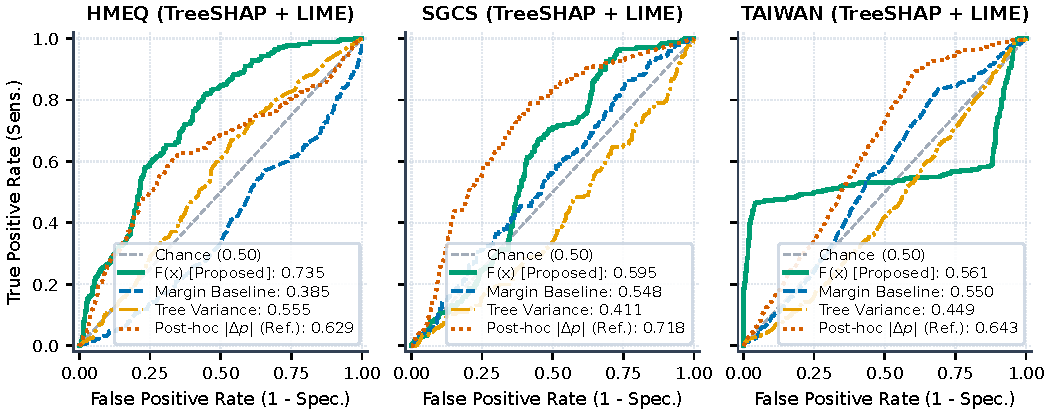
\includegraphics[width=0.49\textwidth]{figures/fig5_roc_comparison.pdf}
\caption{Pooled tree-ensemble ROC curves (TreeSHAP+LIME) predicting instance instability $Y_i$ across HMEQ, SGCS, and Taiwan Default: zero-perturbation ex-ante $F(x)$ vs.\ margin baseline, tree prediction variance, and post-hoc $|\Delta p|$ reference.}
\label{fig:roc_comparison}
\end{figure*}

\subsection{Crossing Mediation and Double Dissociation (H4a--H4c)}
\label{sec:res_h4}
Clustered mediation (Eq.~\eqref{eq:med}, $5{,}000$ instance-cluster bootstraps) confirms H4a in $10/15$ model--explainer cells after Holm--Bonferroni correction ($11/15$ unadjusted): \textbf{all $6/6$ TreeSHAP cells} show large, significant positive indirect effects $a\cdot b$ through $C_{\mathrm{tree}}$ ($p_{\mathrm{Holm}} < 0.001$), including HMEQ \texttt{rf} ($a\cdot b = 1.812$, $95\%$ CI $[1.254, 2.367]$), HMEQ \texttt{xgb} ($3.190$ $[2.630, 3.746]$), SGCS \texttt{rf} ($1.029$ $[0.803, 1.252]$), SGCS \texttt{xgb} ($0.231$ $[0.132, 0.345]$), Taiwan \texttt{rf} ($3.850$ $[3.121, 4.595]$), and Taiwan \texttt{xgb} ($1.949$ $[1.477, 2.407]$). For LIME, $C_{\mathrm{bin}}$ significantly mediates perturbation scale in $4/6$ tree-model cells (HMEQ \texttt{rf}: $0.214, p_{\mathrm{Holm}}=0.007$; HMEQ \texttt{xgb}: $0.110, p_{\mathrm{Holm}}=0.006$; SGCS \texttt{rf}: $0.178, p_{\mathrm{Holm}}<0.001$; SGCS \texttt{xgb}: $0.140, p_{\mathrm{Holm}}<0.001$), whereas LR and Taiwan LIME are masked by sampling noise.

Joint clustered logistic regression on $48{,}547$ tree-model draws across $1{,}178$ instances (Eq.~\eqref{eq:dissoc}; Fig.~\ref{fig:double_dissociation}a) tests double dissociation (H4b). For \textbf{LIME}, the predicted crossover holds cleanly: bin crossings strongly increase flip odds ($\beta_{\mathrm{bin}}=0.309$, $\mathrm{OR}=1.361$ $[1.233, 1.503]$, $p_{\mathrm{Holm}}=2.0\times 10^{-9}$) while tree split crossings have no effect ($\beta_{\mathrm{tree}}=-0.019$, $\mathrm{OR}=0.981$, $p_{\mathrm{Holm}}=0.168$), replicating per dataset on HMEQ ($\beta_{\mathrm{bin}}=0.867, p<10^{-12}$ vs.\ $\beta_{\mathrm{tree}}=0.084, p=0.125$) and SGCS ($\beta_{\mathrm{bin}}=0.823, p=1.5\times 10^{-7}$ vs.\ $\beta_{\mathrm{tree}}=-0.035, p=0.899$). For \textbf{TreeSHAP}, $\beta_{\mathrm{tree}}$ is positive and highly significant across every dataset (pooled $\beta_{\mathrm{tree}}=0.087$, $\mathrm{OR}=1.091$, $p_{\mathrm{Holm}}=7.9\times 10^{-21}$; HMEQ $\beta_{\mathrm{tree}}=0.344, p<10^{-23}$ with non-significant $\beta_{\mathrm{bin}}=0.123, p=0.178$; SGCS $\mathrm{OR}_{\mathrm{tree}}=29.37$ vs.\ $\mathrm{OR}_{\mathrm{bin}}=1.32$), though pooled $\beta_{\mathrm{bin}}=0.171$ ($p_{\mathrm{Holm}}=5.1\times 10^{-10}$) remains nonzero due to residual co-variation in Taiwan continuous-feature neighborhoods. Crucially, the causal intervention H4c (disabling LIME quantile discretisation; Fig.~\ref{fig:double_dissociation}b) cuts mean instability $\bar{U}_i$ by $83.4\%$ on HMEQ ($0.0749 \to 0.0124$, $p=1.09\times 10^{-13}$, $r=0.694$) and $82.1\%$ on SGCS ($0.0818 \to 0.0147$, $p=2.62\times 10^{-16}$, $r=0.693$), with a smaller directional drop on Taiwan ($0.0347 \to 0.0295$, $p=0.072$).

\begin{figure*}[!t]
\centering
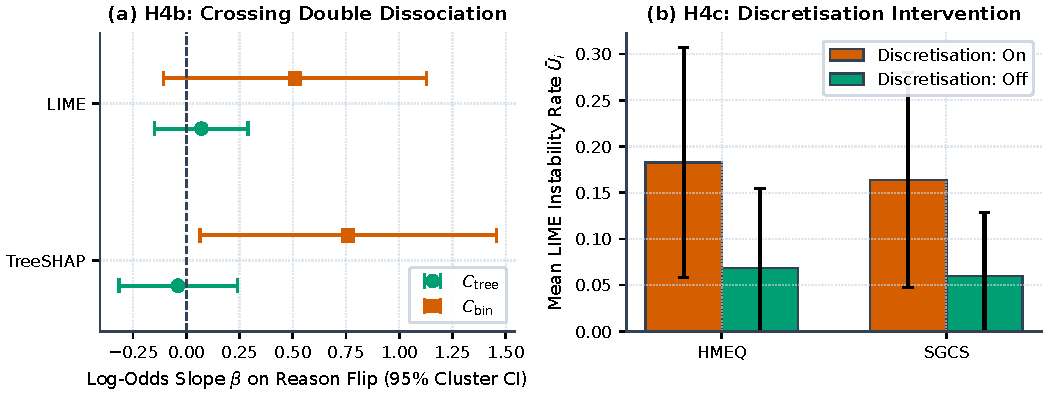
\includegraphics[width=0.49\textwidth]{figures/fig6_double_dissociation.pdf}
\caption{Mechanistic separation of instability sources: (a) H4b double dissociation showing LIME tracks quantile-bin crossings $C_{\mathrm{bin}}$ while TreeSHAP tracks tree split crossings $C_{\mathrm{tree}}$; (b) H4c causal intervention disabling LIME discretisation cuts $\bar{U}_i$ by $>82\%$ on HMEQ and SGCS.}
\label{fig:double_dissociation}
\end{figure*}

\subsection{Ex-Ante Fragility Score (H5) and Exploratory Bridge (H6)}
\label{sec:res_h5h6}
Without running perturbations or holding out a calibration set, closed-form $F(x)$ correlates positively with instance instability $\bar{U}_i$ in $6/6$ TreeSHAP cells ($\rho \in [0.259, 0.531]$, all $p \le 5.5{\times}10^{-4}$). Fig.~\ref{fig:roc_comparison} contrasts pooled tree-ensemble ROC curves (TreeSHAP+LIME) against perturbation-free and $|\Delta p|$ baselines. Across 30 paired DeLong cell comparisons ($15$ cells $\times 2$ baselines), $F(x)$ wins Holm-significantly in $9/30$ cell tests and beats $B_{\mathrm{var}}$ on pooled tree instances across all three datasets: HMEQ ($0.735$ vs.\ $0.555$, $\Delta{=}{+}0.180, p{=}5.1{\times}10^{-14}$), SGCS ($0.595$ vs.\ $0.411$, $\Delta{=}{+}0.184, p{=}7.2{\times}10^{-9}$), and Taiwan ($0.561$ vs.\ $0.449$, $\Delta{=}{+}0.112, p{=}5.9{\times}10^{-5}$), while beating $B_{\mathrm{margin}}$ on HMEQ ($\Delta{=}{+}0.350, p{=}3.2{\times}10^{-40}$) and SGCS ($\Delta{=}{+}0.047, p{=}0.044$). Standout cells include SGCS \texttt{xgb}+TreeSHAP ($0.828$ vs.\ $0.440$ margin, $0.297$ variance, $p_{\mathrm{Holm}}{<}10^{-8}$) and Taiwan \texttt{rf}+TreeSHAP ($0.734$ vs.\ $0.328$ variance, $p_{\mathrm{Holm}}{=}1.5{\times}10^{-8}$); LR+LIME flips remain noise-dominated.

Nested HC3 OLS for H6 ($n{=}3{,}458$) confirms progressive $R^2$ gains from $|\Delta p|$ ($M_1: 0.315{\to}0.345$, $F{=}92.0, p{<}10^{-20}$), empirical crossings ($M_2: {\to}0.360$, $F{=}28.2, p{=}7.0{\times}10^{-13}$), and ex-ante $F(x)$ ($M_3: {\to}0.396$, $F{=}221.1, p{=}1.6{\times}10^{-48}$). Higher IDCS $F_{\mathrm{tree}}(x)$ holds on Taiwan (\texttt{csboost} $0.283$ vs.\ \texttt{xgb} $0.121$, $p{=}2.8{\times}10^{-14}$) but reverses on HMEQ ($0.359$ vs.\ $0.974$) and SGCS ($0.0023$ vs.\ $0.0066$) due to shallower tuned \texttt{csboost} trees (\texttt{max\_depth}=5 vs.\ 7). Table~\ref{tab:hypotheses_summary} consolidates verdicts.

\begin{table}[!t]
\centering
\caption{Summary of Pre-Registered Hypotheses and Empirical Verdicts}
\label{tab:hypotheses_summary}
\scriptsize
\renewcommand{\arraystretch}{0.82}
\setlength{\tabcolsep}{2.4pt}
\begin{tabular}{@{}p{0.8cm}p{4.3cm}p{2.9cm}@{}}
\toprule
\textbf{ID} & \textbf{Key Empirical Evidence} & \textbf{Verdict} \\
\midrule
H1a & $38/40$ ($95.0\%$) Holm-sig.\ ($\tau \in [-0.989, -0.154]$; SGCS \texttt{cslogit}+PermSHAP collapses at $1\%$) & \textbf{Supported (38/40 cells)} \\
H1b & $64/80$ ($80.0\%$) Holm-sig.\ (\texttt{cslogit} $38/40$; \texttt{csboost} $26/40$) & \textbf{Supported (80\% cells)} \\
E1 & LIME balanced $\pi{=}30\%$ explainer share $95.8\%$--$96.2\%$ vs.\ PermSHAP $4.1\%$--$34.3\%$ & \textbf{Quantified (LIME noise-dom.)} \\
H2 & $18/36$ cells ($12/12$ TreeSHAP, $6/6$ LinSHAP; $0/18$ LIME due to high $q_{95}$) & \textbf{Partial (Exact yes; LIME masked)} \\
H3 & $5/12$ full tree cells $<0.70$ (LIME yes; TreeSHAP $0.68$--$0.96$) & \textbf{Not Supported (TreeSHAP); Supported (LIME)} \\
H4a & $10/15$ Holm-sig.\ ($6/6$ TreeSHAP, $4/6$ tree-LIME) & \textbf{Supported (Tree ensembles)} \\
H4b & LIME tracks $C_{\mathrm{bin}}$ ($\mathrm{OR}{=}1.36, p{<}10^{-8}$), not $C_{\mathrm{tree}}$ ($p{=}0.17$); TreeSHAP tracks $C_{\mathrm{tree}}$ ($\mathrm{OR}{=}1.09, p{<}10^{-20}$) & \textbf{Supported (LIME); Partial (TreeSHAP)} \\
H4c & LIME disc.\ OFF cuts $\bar{U}_i$ by $83.4\%$ (HMEQ) \& $82.1\%$ (SGCS, $p{<}10^{-12}$) & \textbf{Supported (HMEQ, SGCS)} \\
H5 & $9/30$ cell Holm-sig.; pooled $F(x)$ beats $B_{\mathrm{var}}$ on all 3 sets ($\Delta\mathrm{AUC}{=}{+}0.11$--$0.18$) & \textbf{Partial (Strong on TreeSHAP)} \\
H6 & $M_0{\to}M_3$ $\Delta R^2{=}{+}0.081$ ($p{<}10^{-47}$); IDCS $F$ higher on Taiwan only & \textbf{Partial (Exploratory)} \\
\bottomrule
\end{tabular}
\end{table}

% ==============================================================================
\section{Robustness Analysis}
\label{sec:robustness}
% ==============================================================================
We evaluate nine robustness checks (R1--R9) spanning structural ablations, tolerance and scale sensitivity, alternative instability definitions, explainer estimation budgets, subgroup and cross-dataset transfer, decision thresholds, and cost-matrix assumptions. Table~\ref{tab:robustness} summarizes every test alongside Fig.~\ref{fig:robustness}, which visualizes nested model ablations (R1) and perturbation-scale monotonicity (R3).

\begin{table}[!t]
\centering
\caption{Summary of Pre-Registered Robustness Checks (R1--R9)}
\label{tab:robustness}
\scriptsize
\renewcommand{\arraystretch}{0.82}
\setlength{\tabcolsep}{2.4pt}
\begin{tabular}{@{}p{0.45cm}p{2.35cm}p{5.1cm}@{}}
\toprule
\textbf{ID} & \textbf{Check} & \textbf{Key Empirical Finding} \\
\midrule
R1 & Nested OLS \& $F(x)$ ablations & $M_0{\to}M_3$ $\Delta R^2{=}{+}0.081$; unweighted $F_{\mathrm{tree}}$ only reaches $\mathrm{AUROC}{=}0.824$ vs.\ cover-wt $0.411$ \& $F_{\mathrm{bin}}$ only $0.219$ \\
R2 & Tolerance $\tau{\in}\{.02,.05,.10\}$ & Pass rate $73.4\%{\to}88.5\%$; $Y_i$ rate $22.3\%{\to}26.1\%$; $F(x)$ AUROC $0.612, 0.611, 0.599$ (invariant) \\
R3 & Scale $s{\in}\{.01,.05,.10\}$ & TreeSHAP $Y_i$ scales ($36.9{\to}59.1{\to}71.7\%$ \texttt{rf}; $33.2{\to}54.5{\to}61.0\%$ \texttt{xgb}); LIME stays flat ($4.4$--$13.8\%$) \\
R4 & Outcomes $D_k, D_\rho, D_1$ \& $k{\in}\{3,4,5\}$ & $\rho(F,\bar{U}_i)$ rises to $0.419$ ($D_\rho$) \& $0.414$ ($D_1$) vs.\ $0.296$ ($D_k$); $k{=}3{\to}5$ preserves $\bar{U}_i \in [0.518,0.549]$ \\
R5 & LIME budget $1\text{k}{\to}5\text{k}$ & $\bar{q}_{95}$ drops $0.494{\to}0.362$ and $\bar{U}_i$ $0.148{\to}0.080$ (HMEQ \texttt{xgb}), yet $\bar{q}_{95}$ remains high \\
R6 & Exact vs.\ PermSHAP & PermSHAP incurs $\bar{q}_{95}\in[0.056,0.284]$, depressing $\bar{U}_i$, while tracking exact TreeSHAP ($\rho{=}0.30$--$0.76$) \\
R7 & Class split \& LODO transfer & $F(x)$ holds in both $y{=}0/1$ (HMEQ $0.744/0.716$); LODO transfers on Taiwan ($85.2\%$ prec., $54.0\%$ rec.) \\
R8 & Threshold $t{=}\text{prior}$ vs.\ $0.50$ & $F(x)$ AUROC ($0.611$ vs.\ $0.609$) \& $\bar{U}_i$ ($0.157$ vs.\ $0.158$) invariant; $B_{\mathrm{margin}}$ drops $0.503{\to}0.421$ \\
R9 & Cost $r_i$ (PV vs.\ $0.02$) & HMEQ/SGCS \texttt{csboost} AUC ($0.907$ vs.\ $0.911$) \& Savings ($0.663$ vs.\ $0.660$) stable \\
\bottomrule
\end{tabular}
\end{table}

\begin{figure*}[!t]
\centering
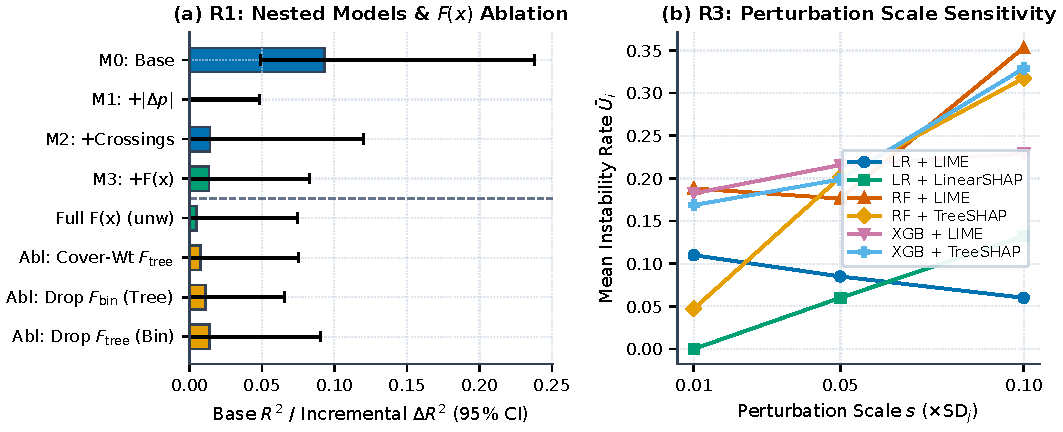
\includegraphics[width=0.49\textwidth]{figures/fig7_robustness_ablation.pdf}
\caption{Robustness diagnostics: (a) R1 nested OLS $\Delta R^2$ progression ($M_0{\to}M_3$) and $F(x)$ component ablations ($95\%$ bootstrap CIs); (b) R3 monotonic scaling of TreeSHAP and LinearSHAP instability across $s \in \{0.01, 0.05, 0.10\}$ vs.\ noise-saturated LIME.}
\label{fig:robustness}
\end{figure*}

\textbf{Structural ablations (R1).} On tree-ensemble instances ($n{=}2{,}862$), isolating $F_{\mathrm{tree}}(x)$ alone raises AUROC from $0.611$ ($F_{\mathrm{tree}}{+}F_{\mathrm{bin}}$) to \textbf{0.824} ($\Delta{=}{+}0.213$, DeLong $p{=}4.1{\times}10^{-62}$) and $\Delta R^2$ to $+0.077$ ($p{=}1.8{\times}10^{-77}$). Cover weighting drops AUROC to $0.411$ ($p{<}10^{-105}$), while $F_{\mathrm{bin}}$ alone yields $0.219$, proving unweighted leaf-path proximity drives TreeSHAP sensitivity.

\textbf{Tolerance, scale, and outcomes (R2--R4).} Varying $\tau{\in}\{0.02,0.05,0.10\}$ shifts pass rate ($73.4\%{\to}88.5\%$) and $Y_i$ rate ($22.3\%{\to}26.1\%$) while $F(x)$ AUROC stays invariant ($0.612,0.611,0.599$). Across $s{\in}\{0.01,0.05,0.10\}$, exact SHAP flip rates scale monotonically (\texttt{rf} $36.9{\to}59.1{\to}71.7\%$; \texttt{xgb} $33.2{\to}54.5{\to}61.0\%$; \texttt{lr} $2.7{\to}10.2{\to}18.5\%$) while LIME stays noise-flat ($4.4\%$--$13.8\%$). Using $D_\rho$ or $D_1$ raises $\rho(F,\bar{U}_i)$ from $0.296$ $[0.261,0.330]$ to $0.419$ and $0.414$; depth $k{\in}\{3,4,5\}$ preserves $\bar{U}_i{\in}[0.518,0.549]$.

\textbf{Budgets, LODO, thresholds, and cost (R5--R9).} Raising LIME samples $1\text{k}{\to}5\text{k}$ on HMEQ \texttt{xgb} lowers $\bar{q}_{95}$ ($0.494{\to}0.362$) and $\bar{U}_i$ ($0.148{\to}0.080$) only partially. PermSHAP (R6) incurs $\bar{q}_{95}{\in}[0.056,0.284]$ while tracking TreeSHAP ($\rho{=}0.30$--$0.76$). Subgroup splits (R7) hold in both classes ($y{=}0/1$: HMEQ $0.744/0.716$; SGCS $0.584/0.623$; Taiwan $0.561/0.561$). Under $t{=}0.50$ (R8), $F(x)$ AUROC is invariant ($0.611$ vs.\ $0.609$) while $B_{\mathrm{margin}}$ drops ($0.503{\to}0.421$). Finally, R9 ($r_i{=}0.02$ vs.\ present-value) leaves IDCS metrics unchanged.

% ==============================================================================
\section{Practical Implications and Case Study}
\label{sec:casestudy}
% ==============================================================================

\subsection{Operational Deployment: Adverse-Action Fragility Gate}
To translate ex-ante fragility diagnostics into consumer-lending operations, we implement an automated reason-code fragility gate in Fig.~\ref{fig:case_study}. After a scoring model issues an adverse decision ($p(x) \ge t$) and an explainer extracts the top-4 principal reasons $T_4(\phi(x))$ aligned with Regulation~B~\cite{regb_cfpb}, the lender evaluates $F(x; s)$ using only model structure and feature standard deviations. Applicants with $F(x) \le \tau_F$ receive standard automated notices, whereas high-fragility applicants ($F(x) > \tau_F$) are routed to manual underwriter review or stabilized local-neighborhood consensus.

\begin{figure}[!t]
\centering
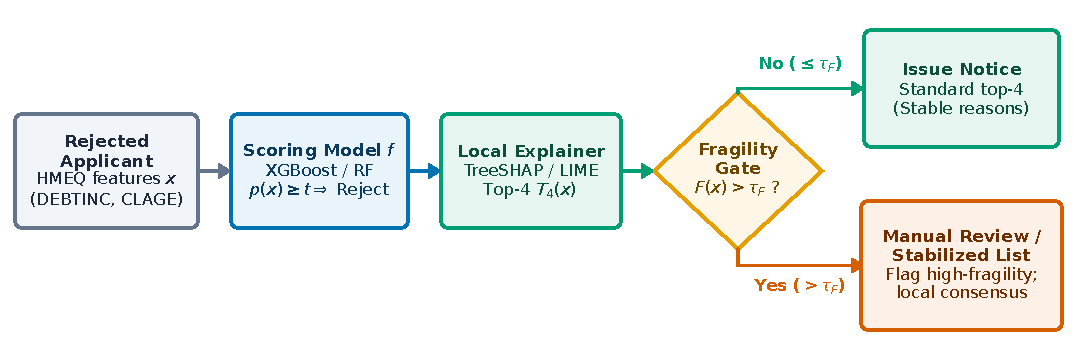
\includegraphics[width=\columnwidth]{figures/fig8_case_study.pdf}
\caption{Operational adverse-action fragility gate workflow for a rejected HMEQ applicant: high-$F(x)$ predictions are routed to manual review or stabilized reason consensus prior to issuing notices.}
\label{fig:case_study}
\end{figure}

\subsection{HMEQ Adverse-Action Walkthrough}
Following our pre-registered selection rule on the HMEQ XGBoost model ($t = 0.1994$, $s = 0.05$, $\tau = 0.05$), Table~\ref{tab:case_study} contrasts the highest-$F_{\mathrm{tree}}$ rejected applicant whose decision and probability remain invariant across all $25$ perturbations (Applicant~\texttt{\#369}) against a low-fragility rejected applicant (Applicant~\texttt{\#166}).

\begin{table}[!t]
\centering
\caption{HMEQ Rejected-Applicant Case Study Walkthrough ($s{=}0.05$, XGBoost)}
\label{tab:case_study}
\scriptsize
\renewcommand{\arraystretch}{0.88}
\setlength{\tabcolsep}{2.6pt}
\begin{tabular}{@{}p{2.2cm}p{2.6cm}p{2.6cm}@{}}
\toprule
\textbf{Attribute / Metric} & \textbf{High-Fragility (\texttt{\#369})} & \textbf{Low-Fragility (\texttt{\#166})} \\
\midrule
Loan / Mortgage & \texttt{LOAN}=\$20k, \texttt{MORTDUE}=\$152k & \texttt{LOAN}=\$7.5k, \texttt{MORTDUE}=\$12.1k \\
Credit History & \texttt{DEROG}=2, \texttt{DELINQ}=5, \texttt{CLAGE}=146.5 & \texttt{DEROG}=3, \texttt{DELINQ}=6, \texttt{CLAGE}=234.9 \\
$p(x)$ / Decision & $0.9999$ (REJECT) & $0.7908$ (REJECT) \\
Ex-ante $F_{\mathrm{tree}}$ / $F_{\mathrm{bin}}$ & \textbf{1.096} / \textbf{1.500} & 0.617 / 0.012 \\
Initial TreeSHAP Top-4 & \texttt{DELINQ}, \texttt{DEROG}, \texttt{DEBTINC}, \texttt{VALUE} & \texttt{DELINQ}, \texttt{DEROG}, \texttt{DEBTINC}, \texttt{CLAGE} \\
Draws $\tau$-preserved & $25/25$ ($100\%$), $\overline{|\Delta p|}{=}0.0036$ & $100\%$ decision preserved \\
Mean $C_{\mathrm{tree}}$ & $1.142$ splits/tree & $0.588$ splits/tree \\
TreeSHAP Flip Rate & \textbf{100.0\%} (\texttt{VALUE} $\leftrightarrow$ \texttt{CLAGE}) & \textbf{0.0\%} (all 4 stable) \\
LIME Flip Rate & $24.0\%$ & $8.0\%$ \\
\bottomrule
\end{tabular}
\end{table}

Applicant~\texttt{\#369} (\texttt{DELINQ}{=}5, \texttt{DEROG}{=}2) is unambiguously rejected ($p{=}0.9999$); across $25$ $5\%$-noise draws, probability barely shifts ($\overline{|\Delta p|}{=}0.0036$) and all draws reject, yet TreeSHAP's fourth reason flips between \texttt{VALUE} ($\phi{=}{+}1.34$) and \texttt{CLAGE} in \textbf{100\% of draws} due to dense split crossings ($C_{\mathrm{tree}}{=}1.142$). Ex-ante $F_{\mathrm{tree}}{=}1.096$ flags \texttt{\#369} \emph{before} perturbations, whereas \texttt{\#166} ($F_{\mathrm{tree}}{=}0.617$, $F_{\mathrm{bin}}{=}0.012$) stays $100\%$ stable ($0\%$ flips). Cross-dataset LODO gating (R7) achieves $85.2\%$ precision and $54.0\%$ recall on held-out Taiwan ($\tau_F{=}0.3285$, $50.0\%$ flagged; $77.1\%$/$57.4\%$ on rejects), whereas unscaled cutoffs over-flag HMEQ ($\tau_F{=}0.0254$: $100\%$ recall, $64.8\%$ overall / $66.9\%$ reject prec.) and under-flag SGCS ($\tau_F{=}13.05$: $0\%$ flagged)—requiring target-portfolio validation-slice calibration.

\subsection{Implications for Model Risk Management}
Ex-ante $F(x)$ complements accuracy and calibration by exposing hidden reason-code fragility on confident denials ($p{=}0.9999$), allowing compliance teams to gate high-$F(x)$ notices and prioritize input verification (e.g., DTI and valuation) without claiming automated legal compliance.

% ==============================================================================
\section{Limitations and Threats to Validity}
\label{sec:limitations}
% ==============================================================================

\subsection{Validity Threats}
\textbf{Construct validity.} Top-4 Jaccard distance ($D_k$) reflects Regulation~B practice~\cite{regb_cfpb} while treating top-4 rank swaps equally; we mitigate this via $D_\rho$, $D_1$, and $k{\in}\{3,5\}$ (R4). Closed-form $F(x)$ assumes independent unclipped Gaussian noise, whereas empirical evaluation validates clipped, $\tau$-filtered draws and unit tests verify unclipped analytical convergence.
\textbf{Internal validity.} Train-only preprocessing, fixed splits, and independent explainer seeds prevent leakage and seed confounding. Omitting \texttt{csforest}, \texttt{net}, and \texttt{csnet} from Part~1 narrows coverage vs.~\cite{ballegeer2025} (Table~\ref{tab:deviations}).
\textbf{External validity.} Findings rest on three public consumer-credit datasets (HMEQ, SGCS, Taiwan) across linear and tree-ensemble models and should not be uncritically extrapolated to deep networks or correlated multi-feature noise.
\textbf{Conclusion validity.} Pre-registered thresholds ($\tau{=}0.05$, $k{=}4$, $\bar{U}_i{\ge}0.20$), Holm--Bonferroni corrections, and $5{,}000$-resample cluster bootstraps guard against multiplicity and within-instance draw correlation.

\subsection{Ethics, Licensing, and Roadmap to Full Conference Submission}
All datasets are anonymized secondary public benchmarks~\cite{baesens2016,sgcs2019,yeh2009} requiring no human-subjects consent, with checksum-verified downloads. Because SGCS contains demographic attributes, local explanation stability does not constitute a fairness audit; subgroup $F(x)$ disparity remains vital future work. Extending this study toward an A* venue (EJOR, AAAI, KDD, or FAccT) will expand coverage to 8--12 datasets, include GPEC and conformal baselines~\cite{hill2024,breeden2026}, and establish formal Lipschitz bounds for $\|\phi(x')-\phi(x)\|_1$.

% ==============================================================================
\section{Conclusion and Future Work}
\label{sec:conclusion}
% ==============================================================================
Replicating Ballegeer et al.~\cite{ballegeer2025} confirmed monotonic instability growth under imbalance ($38/40$ cells) and higher IDCS instability ($64/80$ cells), while variance decomposition proved that $95.8\%$--$96.2\%$ of balanced-data LIME refit variance stems from explainer Monte Carlo noise rather than retraining. Under frozen models and $|\Delta p|\le 0.05$ noise, exact TreeSHAP flips top-4 reasons in $23.5\%$--$92.3\%$ of draws whereas LIME sits beneath its sampling floor ($\bar{q}_{95}\in[0.358,0.722]$). Joint regression across $48{,}547$ tree draws and discretisation ablation proved double dissociation: LIME tracks quantile bins ($\mathrm{OR}{=}1.361$, reduced $>82\%$ without discretisation), while TreeSHAP tracks tree splits ($\mathrm{OR}{=}1.091$). Closed-form fragility $F(x)$ beats tree-variance baselines without perturbations ($\Delta\mathrm{AUROC}{=}{+}0.112$ to $+0.184$), flags HMEQ rejection \texttt{\#369} ($100\%$ flip rate despite $p{=}0.9999$), and invites future target-calibrated thresholds, correlated perturbations, and formal Lipschitz extensions.

\section*{Acknowledgment}
In accordance with course academic integrity guidelines, the authors disclose that AI assistance was utilized solely for grammar checking, LaTeX formatting/debugging, code debugging, and initial research-plan structuring; all experimental execution, verification, and final manuscript authorship were reviewed and owned by the authors.

\section*{Author Contributions (CRediT)}
\textbf{Shahoud Shahid (23i-2515):} Methodology (Part~2 perturbation engine, crossing extraction, closed-form $F(x)$ derivation), Formal analysis (H2--H5, statistical suite), Software, Visualization, Writing---original draft and review. \textbf{Saif Shahzad (23i-2634):} Conceptualization and literature synthesis (gap matrix, BibTeX verification), Methodology (Part~1 replication, IDCS models, E1), Validation (robustness R1--R9), Case study design, Writing---original draft and review.

\bibliographystyle{IEEEtran}
\bibliography{references}

\clearpage
\appendices
\section{Supplementary Audit, Screening, and Baseline Tables}
\label{app:tables}
This appendix documents base-paper alignment choices (Table~\ref{tab:deviations}), feature-level data screening statistics (Table~\ref{tab:screening}), locked software/analysis parameters (Table~\ref{tab:config}), and Part~2 predictive/economic baselines (Table~\ref{tab:model_perf}).

\begin{table}[!t]
\centering
\caption{Replication Alignment and Documented Deviations from Base Paper}
\label{tab:deviations}
\scriptsize
\renewcommand{\arraystretch}{0.86}
\setlength{\tabcolsep}{3.0pt}
\begin{tabular}{@{}p{1.9cm}p{2.6cm}p{3.4cm}@{}}
\toprule
\textbf{Setting} & \textbf{Base Paper~\cite{ballegeer2025}} & \textbf{Our Implementation \& Rationale} \\
\midrule
Datasets & HMEQ, SGCS, GMSC, VUB & HMEQ \& SGCS replicated; VUB omitted (no public URL); Taiwan added \\
Model variants & 8 variants incl.\ \texttt{csforest}, \texttt{net}, \texttt{csnet} & \texttt{logit}, \texttt{cslogit}, \texttt{boost}, \texttt{csboost}, \texttt{forest} (neural/csforest out of scope) \\
Part~1 grid & 8 rates, $J{=}25$ refits & 5 rates $\{1,5,10,20,30\}\%$, $J{=}10$, \texttt{bg}=25, LIME $500$, \texttt{max\_evals}=150 \\
Imputation & Unspecified in manuscript & Train-fold median (numeric) / mode (categorical); zero test leakage \\
SRA formula & Typo in arXiv Eq.~8 ($|S(d)|^2$) & Corrected Ekstr\o m~\cite{ekstrom2019} form verified against Table~4(c) \\
CoV denominator & Signed vs.\ absolute unclear & Absolute mean $|\mu_{ip}|$ (prevents cancellation blow-up) \\
Revenue $r_i$ & Cites Bahnsen~\cite{bahnsen2014} without constants & Vanderschueren~\cite{vanderschueren2022b} annuity formula ($\approx 0.01918\, A_i$) + R9 margin check \\
\bottomrule
\end{tabular}
\end{table}

\begin{table}[!t]
\centering
\caption{Data Screening Summary for Key Continuous and Count Features}
\label{tab:screening}
\scriptsize
\renewcommand{\arraystretch}{0.86}
\setlength{\tabcolsep}{3.0pt}
\begin{tabular}{@{}llrrrrr@{}}
\toprule
\textbf{Dataset} & \textbf{Feature} & \textbf{Missing (\%)} & \textbf{Median} & \textbf{IQR} & \textbf{Outliers (\%)} & \textbf{Skew} \\
\midrule
HMEQ & \texttt{LOAN} & 0.00 & 16,300.0 & 12,200.0 & 4.30 & 2.02 \\
HMEQ & \texttt{MORTDUE} & 8.69 & 65,019.0 & 45,212.0 & 4.30 & 1.81 \\
HMEQ & \texttt{VALUE} & 1.88 & 89,235.5 & 53,748.8 & 5.47 & 3.05 \\
HMEQ & \texttt{CLAGE} & 5.17 & 173.5 & 116.4 & 0.83 & 1.34 \\
HMEQ & \texttt{DEBTINC} & 21.26 & 34.8 & 9.9 & 2.00 & 2.85 \\
\midrule
SGCS & \texttt{duration} & 0.00 & 18.0 & 12.0 & 7.00 & 1.09 \\
SGCS & \texttt{amount} & 0.00 & 2,319.5 & 2,606.8 & 7.20 & 1.95 \\
SGCS & \texttt{age} & 0.00 & 33.0 & 15.0 & 2.30 & 1.02 \\
\midrule
Taiwan & \texttt{LIMIT\_BAL} & 0.00 & 140,000.0 & 190,000.0 & 0.56 & 0.99 \\
Taiwan & \texttt{BILL\_AMT1} & 0.00 & 22,381.5 & 63,532.3 & 8.00 & 2.66 \\
Taiwan & \texttt{PAY\_AMT1} & 0.00 & 2,100.0 & 4,006.0 & 9.15 & 14.67 \\
Taiwan & \texttt{PAY\_AMT2} & 0.00 & 2,009.0 & 4,167.0 & 9.05 & 30.45 \\
\bottomrule
\end{tabular}
\end{table}

\begin{table}[!t]
\centering
\caption{Analysis Configuration and Software Environment}
\label{tab:config}
\scriptsize
\renewcommand{\arraystretch}{0.86}
\setlength{\tabcolsep}{3.0pt}
\begin{tabular}{@{}p{2.7cm}p{5.3cm}@{}}
\toprule
\textbf{Setting} & \textbf{Value / Specification} \\
\midrule
Software & Python 3.11.4 (\texttt{numpy 2.4.4}, \texttt{pandas 3.0.3}, \texttt{scipy 1.17.1}, \texttt{scikit-learn 1.8.0}, \texttt{xgboost 3.2.0}, \texttt{shap 0.51.0}, \texttt{lime 0.2.0.1}, \texttt{statsmodels 0.15.0}) \\
Sample size / coverage & Part~1: $N{=}300$ test/set; Part~2: $n{=}200$ stratified/set ($100\%$ archival data coverage) \\
Missing-data handling & Train-fold median (numeric) and mode (categorical) \\
Estimation methods & MLE/L1-L2 LR; RF; XGB; IDCS (\texttt{cslogit} BFGS, \texttt{csboost} custom AEC objective); HC3 OLS; clustered logit \\
Part~1 settings & $\pi \in \{1,5,10,20,30\}\%$, $J{=}10$ refits, 5-fold CV (iter 1), $\mathrm{SRA}$ depth $d{=}10$, $K{=}5$ E1 repeats, \texttt{bg}=25, LIME $500$, \texttt{max\_evals}=150 \\
Part~2 settings & $t{=}\hat{\pi}_1$, $\tau{=}0.05$, $s \in \{0.01,0.05\}$, $R{=}25$ draws, $K{=}10$ noise-floor repeats, $k{=}4$, background $100$ rows, LIME $1{,}000$ samples \\
Inference & $\alpha{=}0.05$, Holm--Bonferroni correction~\cite{holm1979}, $B{=}5{,}000$ cluster bootstrap resamples, fixed seed $42$ \\
\bottomrule
\end{tabular}
\end{table}

\begin{table}[!t]
\centering
\caption{Part~2 Predictive and Economic Performance vs.\ Base Paper~\cite{ballegeer2025}}
\label{tab:model_perf}
\scriptsize
\renewcommand{\arraystretch}{0.86}
\setlength{\tabcolsep}{2.2pt}
\resizebox{\columnwidth}{!}{%
\begin{tabular}{@{}llrrrrr@{}}
\toprule
\textbf{Data} & \textbf{Model} & \textbf{AUC} & \textbf{AP} & \textbf{Brier} & \textbf{relAEC} & \textbf{Savings} \\
\midrule
Base~\cite{ballegeer2025} & \texttt{boost}/\texttt{csboost} & \textbf{0.837}/0.803 & \textbf{0.556}/0.507 & \textbf{0.102}/0.202 & 0.288/\textbf{0.554} & 0.475/\textbf{0.491} \\
Base~\cite{ballegeer2025} & \texttt{logit}/\texttt{cslogit} & 0.783/0.750 & 0.475/0.371 & 0.117/0.259 & 0.175/0.513 & 0.343/0.431 \\
Base~\cite{ballegeer2025} & \texttt{forest} & 0.821 & 0.526 & 0.115 & 0.167 & 0.449 \\
\midrule
HMEQ & \texttt{lr}/\texttt{cslogit} & 0.782/0.693 & 0.573/0.334 & 0.123/0.236 & 0.207/0.403 & 0.259/0.315 \\
HMEQ & \texttt{rf} & 0.960 & 0.876 & 0.064 & 0.497 & \textbf{0.775} \\
HMEQ & \texttt{xgb}/\texttt{csboost} & \textbf{0.964}/0.931 & \textbf{0.903}/0.819 & \textbf{0.060}/0.086 & 0.624/\textbf{0.672} & 0.707/0.704 \\
\midrule
SGCS & \texttt{lr}/\texttt{cslogit} & 0.743/0.674 & 0.573/0.413 & 0.184/0.326 & 0.320/\textbf{0.551} & 0.061/0.331 \\
SGCS & \texttt{rf} & 0.766 & \textbf{0.596} & 0.172 & 0.225 & 0.347 \\
SGCS & \texttt{xgb}/\texttt{csboost} & \textbf{0.770}/0.713 & 0.581/0.469 & \textbf{0.171}/0.286 & 0.293/0.544 & 0.294/\textbf{0.350} \\
\midrule
Taiwan & \texttt{lr}/\texttt{cslogit} & 0.716/0.670 & 0.498/0.464 & 0.146/0.205 & 0.083/0.322 & 0.184/0.323 \\
Taiwan & \texttt{rf} & 0.775 & \textbf{0.551} & \textbf{0.136} & 0.158 & 0.347 \\
Taiwan & \texttt{xgb}/\texttt{csboost} & \textbf{0.777}/0.702 & 0.548/0.489 & \textbf{0.136}/0.227 & 0.163/\textbf{0.400} & 0.331/\textbf{0.411} \\
\bottomrule
\end{tabular}}
\end{table}

\end{document}
